\documentclass[12pt,twoside,openright,a5paper]{book}

%\usepackage[a5paper, bindingoffset=1cm, inner=2cm, outer=1.5cm]{geometry}
%\usepackage[a5paper]{geometry}
\usepackage[a5paper, hmarginratio={3:2}]{geometry}
%,bindingoffset=1cm
%inner
%outer

\usepackage{times}
\usepackage[Lenny]{fncychap}
%\usepackage[Conny]{fncychap}

\usepackage[spanish]{babel}
\usepackage[utf8]{inputenc}
\usepackage[T1]{fontenc}

\newcommand{\personaje}{Nombre del personaje}

\usepackage{mathptmx}
\usepackage{etoolbox}

\usepackage[titles]{tocloft}

\usepackage{fourier-orns}

\usepackage{graphicx}
\usepackage{float}

\usepackage{soulutf8} % para tachar palabras: \textst{tachame}

\usepackage{pdfpages}
\usepackage{afterpage}

\renewcommand{\cftchapleader}{\cftdotfill{\cftdotsep}}

\hyphenation{a-ttri-bu-tion}
\hyphenation{li-bre-rí-a}
\hyphenation{em-pe-za-ba}
\hyphenation{a-cos-tar-me}
\hyphenation{re-co-rrer}
\hyphenation{ma-yas}
\hyphenation{re-po-llo}
\hyphenation{per-dien-do}
\hyphenation{me-tros}
\hyphenation{di-si-mu-lar}

% Evitar viudas y huérfanas
\widowpenalty=10000
\clubpenalty=10000

\begin{document}

% Quitar los numeros de pagina
\pagenumbering{gobble}

\pagestyle{plain}

%%FOR PRINT
%\includepdf{empty.pdf}
%\includepdf{empty.pdf}
%%%%%%%%%%%

\includepdf{xolopesfirstpage.eps}

%\cleardoublepage

\thispagestyle{empty}
\noindent
Edición automágica, 2013-2014.\\

\vspace{0.5cm}

\noindent
Autor: Juanjo Conti.

\noindent
Corrección: Lis Gariglio.

\noindent
Diseño de la portada: Melisa Puccinelli.

%\noindent
%Fotografías: Cecilia Puccinelli.

\vspace{1cm}

\noindent
\emph{Xolopes} lleva la licencia 
\emph{Creative Commons Attribution - NonCommercial - ShareAlike 3.0 Unported License}.
Esto significa que podés compartir esta obra y crear obras derivadas
mencionando al autor, pero no ha\-cer un uso comercial de ella.

\vfill

\noindent
http://www.juanjoconti.com.ar/xolopes
%Más información sobre este libro: {\small http://www.juanjoconti.com.ar/xolopes}.

\vspace{0.5cm}
\noindent
http://www.juanjoconti.com.ar/libros
%Más libros del autor: {\small http://www.juanjoconti.com.ar/libros}.

\cleardoublepage

\begin{center}
\vspace*{\fill}
\emph{Un libro invisible escrito a la vista de todos.}
\vspace*{\fill}
\end{center}

\cleardoublepage

\noindent
\begin{flushright}
\emph{
\emph{Xolopes} \\está dedicado a mi papá y a mi mamá\\
que me enseñaron a leer \\y a amar.\\
\vspace{0.5cm}
Amo, por eso escribo.
}

\end{flushright}

\cleardoublepage


\hrulefill \hspace{0.1cm}\decofourleft\hspace{0.2cm} 1 \hspace{0.2cm}\decofourright \hspace{0.1cm}\hrulefill

\nopagebreak

\vspace{0.5cm}

\nopagebreak

Conté una ficción en lugar de la realidad para proteger a las personas.

\vspace{0.5cm}

\hrulefill \hspace{0.1cm}\decofourleft\hspace{0.2cm} 2 \hspace{0.2cm}\decofourright \hspace{0.1cm}\hrulefill

\nopagebreak

\vspace{0.5cm}

\nopagebreak

Algunos, un día antes, no saben dónde van a viajar. Entran a un sitio
en Internet, elijen la mejor oferta, manejan hasta el aeropuerto y ¡buen
viaje! Otros, más previsores, nos pasamos cinco meses mirando mapas y
tenemos el viaje pago desde hace tres.

\vspace{0.5cm}

\hrulefill \hspace{0.1cm}\decofourleft\hspace{0.2cm} 3 \hspace{0.2cm}\decofourright \hspace{0.1cm}\hrulefill

\nopagebreak

\vspace{0.5cm}

\nopagebreak

SFE

ROS

EZE

MEX

CUN

PLA

\vspace{0.5cm}

\hrulefill \hspace{0.1cm}\decofourleft\hspace{0.2cm} 4 \hspace{0.2cm}\decofourright \hspace{0.1cm}\hrulefill

\nopagebreak

\vspace{0.5cm}

\nopagebreak

Escuché a dos amigas discutir: 

---¿Y si vamos a un \emph{hostel}?

---Estás loca ---le
dijo una a la otra---. Si vamos a Cancún, vamos a un \emph{all-inclusive}.


\vspace{0.5cm}

\hrulefill \hspace{0.1cm}\decofourleft\hspace{0.2cm} 5 \hspace{0.2cm}\decofourright \hspace{0.1cm}\hrulefill

\nopagebreak

\vspace{0.5cm}

\nopagebreak

El \emph{Heraldo de Quintana Roo} informa: «Ocho detenidos por robo en un hotel
cinco estrellas».

Tres de los apresados son extranjeros. El robo se produjo el domingo a la
noche; se llevaron el dinero de una caja de seguridad ubicada en el
hotel. El botín también incluye joyas de la esposa del dueño.

Fuentes policiales informaron a este medio que un encargado del hotel fue
golpeado y maniatado.

Aparentemente, la caja fuerte no fue violentada e intentan establecer cómo
los ladrones pudieron abrirla sin el código de seguridad.

Se recuperaron algunas joyas del botín, pero el paradero del grueso del
dinero aún es un misterio.

\vspace{0.5cm}

\hrulefill \hspace{0.1cm}\decofourleft\hspace{0.2cm} 6 \hspace{0.2cm}\decofourright \hspace{0.1cm}\hrulefill

\nopagebreak

\vspace{0.5cm}

\nopagebreak

Hay ocasiones en las que los términos medios parecen no existir.
Me acordé de un pasaje de mi infancia: «O frío o caliente, a los tibios los escupiré de mi boca», me citaba a Jesús un
amigo testigo de Jehová cada vez que me ponía dubitativo entre ir o no
a jugar a la pelota.


\vspace{0.5cm}
\afterpage{\includepdf{fotos/pdfs/avion.pdf}}
\hrulefill \hspace{0.1cm}\decofourleft\hspace{0.2cm} 7 \hspace{0.2cm}\decofourright \hspace{0.1cm}\hrulefill

\nopagebreak

\vspace{0.5cm}

\nopagebreak

\hyphenation{a-pa-rez-ca}
\hyphenation{lue-go}
\hyphenation{mi-nu-to}
Auto, colectivo o \emph{transfer}, de una forma u otra, todos llegamos al
aeropuerto. Una vez ahí, a armarse de paciencia. Esperar que el vuelo
aparezca en las pantallas, que no esté retrasado, ir al mostrador,
despachar las valijas, ¿no me habré excedido en el peso? Dieciséis kilogramos, me sobró
lugar. Luego a esperar nuevamente, preembarque, embarque y ahora sí. Estoy
sentado en el avión. Una mole de miles de toneladas de acero alrededor
mío. Ubicado en un reducto ínfimo, incómodo. Miro para los costados y
los demás parecen estar en otro mundo. Algunos juegan con sus teléfonos,
otros miran la pantalla o leen una revista. ¿Cómo pueden estar tan
tranquilos? ¿No se dan cuenta de que en menos de un minuto el capitán va
a encender los motores, o ya los tiene encendidos pero los va a utilizar, y
vamos a pasar todos de estar en la seguridad de tierra firme a estar en la
nebulosa, en un limbo? Ahí pasó una azafata y me pidió que me ajuste el
cinturón y ponga derecho el asiento. Me empiezan a transpirar las manos. El
avión se ubica en la punta de la pista de despegue. Empieza a carretear. No
puedo evitar sentirme en el lomo de un pterodáctilo que corre por la
pista. Aguanto la respiración. Repaso las oraciones de un rosario como si
quisiera ametrallar con mis palabras al pelado de adelante. El corazón me
late. Y ahora, de un momento para otro, dejo de sentir el rugoso asfalto
bajo las ruedas del avión que ya se han despegado de él y lentamente, imagino,
vuelven a formar parte de la mole de acero. Suena una campanita y se apaga
el cartel luminoso que indicaba que nadie podía levantarse. 
«Hemos pasado los diez mil metros de altura», anuncia el capitán.

\vspace{0.5cm}

\hrulefill \hspace{0.1cm}\decofourleft\hspace{0.2cm} 8 \hspace{0.2cm}\decofourright \hspace{0.1cm}\hrulefill

\nopagebreak

\vspace{0.5cm}

\nopagebreak

---\emph{Where are you from, girls?}

---Argentina.

---\emph{Where is that? Somewhere in Mexico?}

\vspace{0.5cm}

\hrulefill \hspace{0.1cm}\decofourleft\hspace{0.2cm} 9 \hspace{0.2cm}\decofourright \hspace{0.1cm}\hrulefill

\nopagebreak

\vspace{0.5cm}

\nopagebreak

Al final fuimos a un \emph{all-inclusive}. Una pulserita, comida y bebida gratis en abundancia, todo el día, todos los días.

Yo me consolaba solo diciéndome que así ya tenía resuelto el tema de
la comida. Soy celíaco, intolerante a la lactosa, abstemio y tengo colon
irritable. No pude comer nada.


\vspace{0.5cm}

\hrulefill \hspace{0.1cm}\decofourleft\hspace{0.2cm} 10 \hspace{0.2cm}\decofourright \hspace{0.1cm}\hrulefill

\nopagebreak

\vspace{0.5cm}

\nopagebreak

Vas caminando por un bosque oscuro, sentís una presencia a tu espalda
y en lugar de darte vuelta, empezás a correr y a correr. Te tropezás,
caés, te levantás y seguís corriendo. La presencia, atrás, está cada vez
más cerca. Adelante ves un precipicio, no tenés tiempo siquiera
para pensarlo, seguís corriendo hasta que saltás. Mientras vas cayendo, te
despertás. Estás en el asiento del avión. Otra vez te dormiste y otra vez
te despertaste. Mirás el reloj; es la tercera vez en la última hora. Notás
movimiento unas filas más adelante; un hombre grande y rubio se mueve  como
si lo estuvieran electrocutando. Las personas de los asientos contiguos
se levantan asustadas. Más movimiento. Una azafata te pasa por al lado
corriendo. Escuchás al capitán preguntar si hay un médico a bordo. El
viejito sentado dos lugares más allá se levanta. Ahora, el hombre rubio
está tirado en el piso del avión. Alguien le practica técnicas de
reanimación. Ves cómo arrastran al hombre rubio detrás de
unas cortinas.

\vspace{0.5cm}

\hrulefill \hspace{0.1cm}\decofourleft\hspace{0.2cm} 11 \hspace{0.2cm}\decofourright \hspace{0.1cm}\hrulefill

\nopagebreak

\vspace{0.5cm}

\nopagebreak

Lo lindo de tomar excursiones es que te sale más caro que si vas por tu
cuenta. Te buscan a las siete de la mañana, pero hasta las diez no dejan la ciudad (hay que
buscar al resto de los excursionistas) y, una vez en el destino, no tenés
tiempo de recorrer tranquilo porque el guía te va ametrallando datos que
no vas a recordar a la salida del lugar. No.

\vspace{0.5cm}

\hrulefill \hspace{0.1cm}\decofourleft\hspace{0.2cm} 12 \hspace{0.2cm}\decofourright \hspace{0.1cm}\hrulefill

\nopagebreak

\vspace{0.5cm}

\nopagebreak

Ayer, de pasada, escuché a dos mozos hablar sobre el agujero de la cerradura de
una de las habitaciones. No alcancé a escuchar exactamente a qué habitación
se referían, pero decodifiqué un «setecientos cuarenta y...» y vi que uno
de los dos hacía gestos obscenos mientras el otro se reía a carcajadas. 
En un día nublado y con lloviznas en la península de Yucatán y sin nada 
que hacer, dejé el área de desayuno y me fui caminando hasta el bloque 7.

\vspace{0.5cm}

\hrulefill \hspace{0.1cm}\decofourleft\hspace{0.2cm} 13 \hspace{0.2cm}\decofourright \hspace{0.1cm}\hrulefill

\nopagebreak

\vspace{0.5cm}

\nopagebreak

\emph{Chichén Itzá. Vocablo maya. Chichén: \emph{boca del pozo}. Itzá: \emph{brujos de agua}.
Es uno de los principales sitios arqueológicos de la península de Yucatán,
en México, ubicado en el municipio de Tinum, en el estado de Yucatán.}

\vspace{0.5cm}
\afterpage{\includepdf{fotos/pdfs/hotel.pdf}}
\hrulefill \hspace{0.1cm}\decofourleft\hspace{0.2cm} 14 \hspace{0.2cm}\decofourright \hspace{0.1cm}\hrulefill

\nopagebreak

\vspace{0.5cm}

\nopagebreak

Volvés a escuchar la voz del capitán. «Les habla su capitán. Hay una
persona descompuesta y no estamos pudiendo ayudarla, por lo que vamos a
lanzar el combustible al mar y aterrizar en Recife». Sentís la fuerza del
avión regresando. Media hora después, aterrizan. Más movimiento. No pasan
cinco minutos cuando volvés a oír al capitán. «Les habla su capitán.
Lamentablemente tengo que informarles que el pasajero murió».

\vspace{0.5cm}

\hrulefill \hspace{0.1cm}\decofourleft\hspace{0.2cm} 15 \hspace{0.2cm}\decofourright \hspace{0.1cm}\hrulefill

\nopagebreak

\vspace{0.5cm}

\nopagebreak

\hyphenation{cons-ti-tu-ción}
\hyphenation{sec-ción}

Al llegar al hotel,
mientras nos llevan junto a nuestras valijas en un carrito de golf hasta
la zona de las habitaciones, vemos una escena curiosa. Un simpático personaje
(luce la misma ropa que el chofer del carrito de golf, aunque es claramente
más viejo) está parado sobre un banquito (como casi todos los empleados,
apenas si supera el metro cincuenta) hablando a través de un megáfono.

---No existe, compañeros, una ley específica sobre salarios mínimos en
México. Sin embargo... Sin embargo, en la Constitución Política de México,
Art. 123, Sección VI, se encuentra el sustento legal para nuestros
salarios mínimos generales, compañeros. Es principalmente la Ley Federal
del Trabajo la que contiene la regulación de los salarios mínimos.
Entre los Art. 90 y 97, están sus características principales.

»El salario mínimo en México es de 60,66 dólares diarios, lo que equivale
a 4,4 dólares. Esto resulta insuficiente para cubrir las necesidades de una
familia. En la constitución mexicana, compañeros, se determina que la 
Comisión Nacional de Salarios
Mínimos, integrada por el gobierno más empleadores y trabajadores, será la
responsable... será la responsable de fijar los salarios mínimos cada
año. A pesar de este esquema, el salario mínimo ha perdido un 80\% de su
poder adquisitivo desde 1882.

---¿Quién es ese? ---le pregunto al conductor.

---¿Ese? Ese es el viejo Gaspar.


\vspace{0.5cm}

\hrulefill \hspace{0.1cm}\decofourleft\hspace{0.2cm} 16 \hspace{0.2cm}\decofourright \hspace{0.1cm}\hrulefill

\nopagebreak

\vspace{0.5cm}

\nopagebreak

\hyphenation{mo-ne-da}
---En el último grupo que traje había un hombre que me mostraba contento
unas monedas que le habían dado de cambio en uno de los puestos de
artesanías. «Dólares maya», le dijeron. «Un dólar americano, un dólar maya». Eran
quetzales, la moneda de Guatemala. Tengan cuidado.

\vspace{0.5cm}

\hrulefill \hspace{0.1cm}\decofourleft\hspace{0.2cm} 17 \hspace{0.2cm}\decofourright \hspace{0.1cm}\hrulefill

\nopagebreak

\vspace{0.5cm}

\nopagebreak

\emph{El mar y la playa son como un libro inmenso, un libro infinito, que día
a día va pasando sus páginas. Cada ola sobre la arena que trae algo y se
lleva un poco puede verse como una hoja de ese libro que alguien va pasando.}

\emph{Los glifos con los que se escribe son marcas en la arena. Un cuadrado que
delimita una cancha, un corazón que dice \mbox{J y C}, un castillo.}

\vspace{0.5cm}

\hrulefill \hspace{0.1cm}\decofourleft\hspace{0.2cm} 18 \hspace{0.2cm}\decofourright \hspace{0.1cm}\hrulefill

\nopagebreak

\vspace{0.5cm}

\nopagebreak

\hyphenation{pa-si-llo}
Una vez en el bloque 7, subí las escaleras hasta el piso 4 y,
mirando el amplio pasillo, me puse a pensar cuál de los picaportes sería el
custodio del entretenimiento de los mozos. Sin nada que me dé una señal,
empecé a apoyar la oreja en cada una de las puertas.

Estaba apoyado bajo un lustroso número setecientos cuarenta y cuatro cuando la superficie que me
sostenía se esfumó. La puerta se había abierto y yo caí, despatarrado
y haciendo mucho ruido, a los pies de una señorita de zapatos rojos con
taco aguja.

\vspace{0.5cm}

\hrulefill \hspace{0.1cm}\decofourleft\hspace{0.2cm} 19 \hspace{0.2cm}\decofourright \hspace{0.1cm}\hrulefill

\nopagebreak

\vspace{0.5cm}

\nopagebreak

Caminando por Tulum:

---Podemos acortar camino por acá; lo que no está
prohibido está permitido.

\vspace{0.5cm}

\hrulefill \hspace{0.1cm}\decofourleft\hspace{0.2cm} 20 \hspace{0.2cm}\decofourright \hspace{0.1cm}\hrulefill

\nopagebreak

\vspace{0.5cm}

\nopagebreak

\hyphenation{bra-si-le-ño}
\hyphenation{e-xi-ge}
\hyphenation{via-je}
%Pasó una hora y el clima en el avión es tenso. 
Después de haber pasado una hora, el clima del avión es tenso. 
Te preguntás qué mierda
estará pasando cuando volvés a escuchar la voz del capitán. 
«Les habla
su capitán. Tengo que informarles que se ha encontrado cocaína en las
pertenencias del pasajero y la policía local no nos permite continuar el
viaje hasta realizar los peritajes necesarios en el avión».

Ves a un padre
con su bebé en brazos a las puteadas. Lo mandan a primera clase, igual que
hicieron con los que estaban en la misma fila que el hombre rubio. Suben
oficiales de policía al avión, sacan fotos al asiento del pasajero muerto,
toman muestras y, por último, se llevan la funda del asiento. Pasan dos
horas más y el capitán anuncia que aún no han conseguido combustible para
reponer el volcado en el océano. Es probable que tengan que dejar el avión,
pasar la noche en un hotel y continuar al día siguiente. Un brasileño se
ríe. 

---Es que ---te cuenta--- Brasil le exige visa a los norteamericanos igual
que Estados Unidos le exige visa a los brasileños. Los van a hacer renegar
un buen rato ---te dice.

\vspace{0.5cm}

\hrulefill \hspace{0.1cm}\decofourleft\hspace{0.2cm} 21 \hspace{0.2cm}\decofourright \hspace{0.1cm}\hrulefill

\nopagebreak

\vspace{0.5cm}

\nopagebreak

\hyphenation{in-sig-ni-fi-can-te}
\hyphenation{re-cep-cio-nis-tas}
\hyphenation{be-ach}
\hyphenation{mo-chi-la}
---De toda la fauna humana que se puede ver rebotando por Playa del Carmen, uno
de los especímenes más curiosos son los mochileros. Hombres o mujeres,
en su mayoría de entre veinte y treinta años (aunque hay excepciones), que se
trasladan de una ciudad a otra, de un país a otro o de un continente a
otro, cargando en sus espaldas todo lo que necesitan para subsistir. Estos
caracoles humanos se caracterizan por intentar gastar la menor cantidad de
dinero posible a la vez que maximizan las experiencias vividas. Su lugar
predilecto para pernoctar son los \emph{hostels} en el centro de la ciudad, pero
si alguien les ofrece techo a cambio de trabajo o algún tipo de acuerdo
similar, no dudan en aceptar.

»Si los clasificamos por su modo de viajar, podemos distinguir dos grupos
principales: los ahorristas y los buscavidas. El primer grupo suele viajar
durante períodos de tiempo más cortos y cuando se les termina el dinero
ahorrado para el viaje, vuelven a su lugar de origen, trabajan por un
tiempo determinado y vuelven a salir a la aventura. El segundo grupo está
formado por personas que alguna vez fueron ahorristas pero se cansaron
de tener que interrumpir constantemente el viaje de la vida por algo tan
insignificante como el dinero. Es por eso que en un punto del camino
deciden no regresar y encuentran formas alternativas de vivir, bajan sus
expectativas de confort y sus travesías duran años. Los hay malabaristas,
vendedores, recepcionistas...

»¿Yo? No, yo estoy parando en el \emph{Ocean Beach Caribbean Resort}. No, nunca
salí con la mochila. Vi lo que estoy contando en un documental.

\vspace{0.5cm}
\afterpage{\includepdf{fotos/pdfs/mochila.pdf}}
\hrulefill \hspace{0.1cm}\decofourleft\hspace{0.2cm} 22 \hspace{0.2cm}\decofourright \hspace{0.1cm}\hrulefill

\nopagebreak

\vspace{0.5cm}

\nopagebreak

\hyphenation{mi-nu-tos}
\hyphenation{la-bo-ra-les}
Bitácora de la \st{revolución} rebelión. Día 1. Hoy, durante la hora libre, que en
realidad son cuarenta y seis minutos, nos hemos reunidos con los compañeros alineados
a la causa con el objetivo de trazar líneas de acción, orientadas a poner
en marcha un plan que nos permita obtener las mejoras laborales que venimos
reclamando durante los últimos años y que la administración del hotel
se ha negado sistemáticamente a concedernos. A saber:

\begin{enumerate}
\item reducción de la jornada laboral de catorce a nueve horas con una hora de descanso;
\item aumento del salario mínimo de mil trecientos pesos a cinco mil pesos.
\end{enumerate}

Como la negativa ya fue afirmada y reafirmada, hemos decidido recuperar
estos derechos a la fuerza. Aunque «a la fuerza» tal vez no sea la expresión
correcta. Utilizaremos más bien el ingenio. Nos vamos a valer de los turistas
para lograr nuestro objetivo.

\vspace{0.5cm}

\hrulefill \hspace{0.1cm}\decofourleft\hspace{0.2cm} 23 \hspace{0.2cm}\decofourright \hspace{0.1cm}\hrulefill

\nopagebreak

\vspace{0.5cm}

\nopagebreak

\hyphenation{se-ña-la-ba}
La chica que me miraba desde su altura más la de los veinte centímetros de
los tacos me empezó a hablar en una lengua que no reconocí. Me levantó
del hombro (era muy fuerte y, sumado a la pista del idioma, intuí que era rusa o
ucraniana, medallista olímpica de lanzamiento de martillo, ¿por qué
no?). Evidentemente se pensó que yo era personal de maestranza o algo
parecido, porque con unas palabras que adiviné como insultos me señalaba
el reloj y a los empujones me llevó hasta el baño de la habitación donde
cataratas de agua emanaban por todos los elementos de grifería.

\vspace{0.5cm}

\hrulefill \hspace{0.1cm}\decofourleft\hspace{0.2cm} 24 \hspace{0.2cm}\decofourright \hspace{0.1cm}\hrulefill

\nopagebreak

\vspace{0.5cm}

\nopagebreak

«Les habla su capitán. Les informo que hemos podido reabastecernos
del combustible necesario para continuar el viaje. En cuarenta minutos
iniciaremos el despegue».
Ya pasaron seis horas desde el aterrizaje y es
de noche. La mayoría de los pasajeros están dormidos y vos, desvanecido,
te dormís cuando el avión está despegando.

\vspace{0.5cm}

\hrulefill \hspace{0.1cm}\decofourleft\hspace{0.2cm} 25 \hspace{0.2cm}\decofourright \hspace{0.1cm}\hrulefill

\nopagebreak

\vspace{0.5cm}

\nopagebreak

\hyphenation{chan-gas} \hyphenation{des-en-ros-can-do} Acostumbrado a
arreglar las cosas en casa, me arremangué para revisarle la cañería a
la señorita. (Por favor, absténganse de malos pensamientos que esta no es ese
tipo de historias). Estuve escarbando, destrabando, soplando, desenroscando,
girando, palpando, doblando, estirando, sacudiendo, estrujando y reensamblando
alrededor de media hora hasta que en una de las secciones de la cañería
encontré, atascado, cien kilos de papel higiénico y descartables de aseo
personal, varios condensados en una pelota de cinco centímetros de diámetro.

Como un héroe que rescata una mascota, se la mostré a la ucraniana (ya la
había bautizado así en mis pensamientos) y me hizo cara de asco. Tiré
la pelota en el cesto de la basura y procedí a lavarme las manos, los
antebrazos, los codos, los brazos y hasta la nuca; era una limpieza sin fin.
Una vez presto y rechinando de limpio, volví mi atención a la señorita. El
agua ya no brotaba a borbotones y su pesadilla cloacal parecía haber terminado.
Me tomó de las manos y vi en sus ojos el deseo de agradecerme. Casi
lágrimas le provocaba la emoción y la impotencia de no poder hablarme en
mi idioma natal. Miró con el rabillo del ojo la cama matrimonial y a mí
se me aceleró el corazón. En ese momento escuché la llave, el picaporte
y la puerta.

\vspace{0.5cm}

\hrulefill \hspace{0.1cm}\decofourleft\hspace{0.2cm} 26 \hspace{0.2cm}\decofourright \hspace{0.1cm}\hrulefill

\nopagebreak

\vspace{0.5cm}

\nopagebreak

Caminando por Tulum:

---Vamos a descansar un rato porque todavía tenemos que
caminar «del dicho al hecho».

\vspace{0.5cm}

\hrulefill \hspace{0.1cm}\decofourleft\hspace{0.2cm} 27 \hspace{0.2cm}\decofourright \hspace{0.1cm}\hrulefill

\nopagebreak

\vspace{0.5cm}

\nopagebreak

\hyphenation{pa-sa-je-ro}
\hyphenation{e-llas}
\hyphenation{fe-de-ral}
El \emph{Folha de S. Paulo} informa: «Africano muere
durante vuelo con ciento cuatro cápsulas de cocaína en el estómago».

El sudafricano
Louis Hendrik Smith, de treinta y cuatro años, murió esta tarde durante un vuelo entre
Argentina y México, se presume por sobredosis de cocaína. Fuentes de
la Policía Federal informan que Smith había ingerido 1,7 kg de droga,
divididos en ciento cuatro cápsulas. Una de ellas, con cerca de dieciséis gramos de sustancia,
se rompió en el estómago del pasajero.

Luego de un aterrizaje de emergencia, el pasajero fue atendido por dos
médicos, pero estos no pudieron hacer nada porque ya estaba muerto.

Las autoridades policiales retiraron el equipaje del pasajero del avión y
liberaron a los restantes trecientos ocho pasajeros y diecisiete tripulantes para que continúen
su viaje a las doce de la noche.  Según la superintendencia de la Policía
Federal, todo indicaría que la víctima compró e ingirió la droga en
la Argentina.

\vspace{0.5cm}
\afterpage{\includepdf{fotos/pdfs/chichen.pdf}}
\hrulefill \hspace{0.1cm}\decofourleft\hspace{0.2cm} 28 \hspace{0.2cm}\decofourright \hspace{0.1cm}\hrulefill

\nopagebreak

\vspace{0.5cm}

\nopagebreak

\hyphenation{hu-ma-ni-dad}
La zona arqueológica de Chichén Itzá fue inscripta en la lista del
Patrimonio de la Humanidad por la Unesco en 1988. El 7 de julio de 2007 fue
reconocida como una de las nuevas siete maravillas del mundo moderno por
una iniciativa privada sin el apoyo de la Unesco, pero con el reconocimiento
de millones de votantes alrededor del mundo.

Desde ese día no está permitido subirla.

\vspace{0.5cm}

\hrulefill \hspace{0.1cm}\decofourleft\hspace{0.2cm} 29 \hspace{0.2cm}\decofourright \hspace{0.1cm}\hrulefill

\nopagebreak

\vspace{0.5cm}

\nopagebreak

\hyphenation{cua-tro}
\hyphenation{ce-rra-du-ra}
\hyphenation{Schwarz-en-egger}
\hyphenation{Arn-old}
No miento si digo que podría ser doble de riesgo de Arnold Schwarzenegger. El
marido de la ucraniana era tan ancho de espalda como yo de alto. Tenía
una malla celeste con flores verde flúo y un toallón colgado de la
espalda. Cuando me vio, el rostro se le transformó y empezó a gritarle a
su mujer. Puteadas en ucraniano, supongo, \emph{obolonka tvoyei sestry, ty suka,
podyvit'sya na mudaka Ty shcho, zhartuyesh}. Después me miró a mí. Tenía
la piel roja por el calor del momento y me mostró su dentadura lobuna. Voy
a resumir lo siguiente que pasó diciendo que me hizo todo lo que yo le
hice a las cañerías de su habitación, pero con menos delicadeza. Cuando
pude escaparme y salir de la setecientos cuarenta y cuatro, me encontré a
los mozos espiando por la cerradura, muertos de risa.

\vspace{0.5cm}

\hrulefill \hspace{0.1cm}\decofourleft\hspace{0.2cm} 30 \hspace{0.2cm}\decofourright \hspace{0.1cm}\hrulefill

\nopagebreak

\vspace{0.5cm}

\nopagebreak

\hyphenation{Mé-xi-co}
Algo que no conté del tipo del avión es que, cuando me subí, estaba
sentado en mi asiento, el 32B. Se confundió; el suyo era el 23B. Cuando
me desperté, con todo el movimiento, no me di cuenta, pero antes de bajarme
la vi; debajo del 32B, estaba su billetera. Me di cuenta por las fotos en
las credenciales. Ya estábamos en México, ¿qué iba a hacer? ¿Llevarla
a la policía?, ¿la policía de México se la iba a llevar a la policía
de Brasil?, ¿a la de Sudáfrica? Mucha logística y yo estaba arrancando
las vacaciones. Me la guardé en la mochila para después tirarla. Sí,
es verdad. No suelo tomar las mejores decisiones.

\vspace{0.5cm}

\hrulefill \hspace{0.1cm}\decofourleft\hspace{0.2cm} 31 \hspace{0.2cm}\decofourright \hspace{0.1cm}\hrulefill

\nopagebreak

\vspace{0.5cm}

\nopagebreak

Vengo caminando desprevenido y ataca un vendedor.

---\emph{One dollar}.

Lo corto en seco y sigo caminando:

---No hay plata.

---¿Argentino? Mitad de precio. Algo para la suegra. ¡Un recuerdito! ---me grita
para que lo escuche.

Me doy vuelta y contesto:

---No se lo merece.

El tipo sonríe mostrando los dientes que le faltan y remata: 

---También tenemos cuchillos.

\vspace{0.5cm}

\hrulefill \hspace{0.1cm}\decofourleft\hspace{0.2cm} 32 \hspace{0.2cm}\decofourright \hspace{0.1cm}\hrulefill

\nopagebreak

\vspace{0.5cm}

\nopagebreak

\hyphenation{ca-ri-be}
\hyphenation{su-pues-to}
\hyphenation{si-llón}
\hyphenation{se-ñas}
\hyphenation{in-su-pe-ra-ble}
\hyphenation{li-mi-tó}
\hyphenation{a-gra-da-ble}
\hyphenation{la-ti-no-a-me-ri-ca-no}
\hyphenation{quie-nes}
\hyphenation{mar-tín}
\hyphenation{co-la-te-ra-les}
Hace unos años leí esta historia en un post en el blog de Fede Heinz;
¿lo tenés? El de barba y pelo largo. Bueno, te decía que me acordé de
esta historia. Te la paso porque te puede servir para la novela:

«En el primer día de sus vacaciones en el Caribe, Martín salió a matar. De
abajo para arriba, llevaba ojotas, bermudas rojas, camisa floreada, amplia
para disimular la ``zapán'' y abierta para que se viera la cadena de oro,
anteojos negros con marco de metal dorado y la gorra del Club Atlético
Talleres (no por seductor iba a renegar de sus sentimientos más
profundos). Entró en la playa con el pecho henchido, consciente de que las
minas lo miraban. Con su andar recio, tirando arena para arriba con el
talón de las ojotas a cada paso, se dirigió a un sillón de playa sobre
el que se recostó con un profundo suspiro de placer.

Tanto despliegue de masculinidad, por supuesto, no podía pasar desapercibido;
 al fin y al cabo, las mujeres tampoco son de palo y menos en esas
latitudes en las que el sol y la naturaleza mantienen la sangre siempre
efervescente. Había estado escasos minutos sobre el sillón cuando escuchó
una voz melódica que le preguntaba ``\emph{Would you mind spreading some sun
lotion on my back?}''. Martín no hablaba una palabra de inglés, lo que no
le impidió comprender la pregunta, porque pocas cosas hay más cercanas a
un lenguaje universal que la imagen de una morena pechugona, apenas cubierta
por una minúscula tanga, extendiendo un frasco de bronceador con la mano
derecha, al tiempo que, con la izquierda, se frota demostrativamente el
hombro opuesto. Haciendo un enorme y fútil esfuerzo por mantener la calma,
Martín se levantó y procedió a esparcir el bronceador sobre el dorso de la
ninfa. Ella festejaba con leves gemidos de placer cada uno de sus movimientos,
que iban haciéndose cada vez menos enérgicos y amplios a medida que él
se daba cuenta de que, a ese ritmo, la espalda se le acabaría enseguida.

Como muestra de agradecimiento, y por señas, ella le ofreció
compartir con él un trago en el bar de la playa. Allí, en virtud de la
insuperable barrera idiomática, la conversación se limitó a un constante
intercambio de sonrisas que, ocasionalmente, estallaba en inexplicables
carcajadas. Brindaron, bebieron el uno de la copa del otro, se hicieron caras
y sin previo aviso, Martín se encontró con un pie de ella suavemente apoyado
en su entrepierna, lo que cambió de inmediato la naturaleza de su sonrisa.

No habían aún terminado el segundo trago cuando se acercó a la mesa
otra muchacha, más hermosa, exuberante y desnuda que la primera (si tal
cosa cabía), quien saludó a la morena con un beso en la boca. Intercambiaron breves
frases en inglés, lanzando de vez en cuando risitas y miradas pícaras en
dirección a Martín. De alguna manera, se las arreglaron para preguntarle
al oído si no quería acompañarlas a la habitación del hotel, donde las
estaba esperando otra amiga.

El hotel no estaba lejos y la puerta se abrió para revelar a la más bella,
 voluptuosa y desnuda de las tres, quien los esperaba con tragos
servidos. Martín tardó un momento en darse cuenta de la presencia de otro
hombre en la habitación y, pese a que su aspecto era agradable, sintió
cierto temor. El extraño resultó ser un centroamericano muy cordial,
de nombre Carlos, que al ver que Martín no hablaba inglés, inició una
charla con él para que no se sintiera tan aislado.

Comenzó hablándole de la belleza del hotel y de la comodidad de las
habitaciones. Mientras una de las chicas abrazaba a Martín por detrás,
metiendo su mano bajo la camisa para pellizcarle las tetillas, Carlos alababa
las artes de los cocineros y observaba las ventajas de estar tan cerca de
la playa. Tironeado entre sus sentimientos de urbanidad y solidaridad que le
impedían dejar hablando solo a un hermano latinoamericano y su libido
que constantemente le hacía desviar la vista hacia las otras dos amigas
que se besaban y acariciaban sobre el sofá, Martín simulaba escuchar
las apreciaciones de Carlos acerca del impecable servicio de seguridad y
la altísima calidad de la atención, comparable solo a la de los hoteles
cinco estrellas.

Martín pasó todo el día siguiente tratando de reconstruir cómo y por qué
había salido de la habitación sin siquiera haber tocado a las niñas, pero
sobre todo no conseguía recordar en qué momento había firmado el contrato
que lo hacía acreedor, por las siguientes dos décadas, a una habitación
del hotel en tiempo compartido, diez días al año, del 3 al 13 de junio,
por una módica cuota mensual más servicio de mucama, seguros, gastos
comunes, administrativos y colaterales, sellados, prima de mantenimiento,
comisiones e impuestos».

\vspace{0.5cm}

\hrulefill \hspace{0.1cm}\decofourleft\hspace{0.2cm} 33 \hspace{0.2cm}\decofourright \hspace{0.1cm}\hrulefill

\nopagebreak

\vspace{0.5cm}

\nopagebreak

---¿Lo viste al flaco ese? Un solo machucón. Para mí que se cayó de la
pirámide de Cobá.


\vspace{0.5cm}
\afterpage{\includepdf{fotos/pdfs/coba.pdf}}
\hrulefill \hspace{0.1cm}\decofourleft\hspace{0.2cm} 34 \hspace{0.2cm}\decofourright \hspace{0.1cm}\hrulefill

\nopagebreak

\vspace{0.5cm}

\nopagebreak

\hyphenation{a-dre-na-li-na}
\hyphenation{cual-quier}
En mi quinta noche en México, solo en la habitación del hotel, me acordé
de la billetera del sudafricano, la «mula». Cualquier persona la hubiese
dejado ahí, en el piso del avión, o se la hubiese dado a una azafata
y listo. Señorita, encontré esto en mi asiento; tome; gracias; no, de
nada. Listo, chau, vacaciones. Pero yo no, siempre tuve esa enfermedad de
creerme detective o policía o a veces ladrón. Esa necesidad de adrenalina,
teórica, porque si veo un arma o sangre, seguro me meo encima.

\vspace{0.5cm}

\hrulefill \hspace{0.1cm}\decofourleft\hspace{0.2cm} 35 \hspace{0.2cm}\decofourright \hspace{0.1cm}\hrulefill

\nopagebreak

\vspace{0.5cm}

\nopagebreak

Paseando por Chichén Itzá, otro vendedor de estatuitas nos grita mientras
pasamos:

---Chica, elija el que le gusta, el chico paga.

\vspace{0.5cm}

\hrulefill \hspace{0.1cm}\decofourleft\hspace{0.2cm} 36 \hspace{0.2cm}\decofourright \hspace{0.1cm}\hrulefill

\nopagebreak

\vspace{0.5cm}

\nopagebreak

\hyphenation{di-rec-ción}
En la billetera del sudafricano, al que le explotó la cápsula
de cocaína adentro, encontré cuatrocientos dólares, identificaciones y una
tarjeta. La tarjeta era blanca y en letras de molde negras tenía tatuada
una dirección. Del otro lado, tenía el dibujo de un ángel con las alas
rotas. La dirección era en Cancún, en un lugar alejado de la línea de
hoteles. Una tarde me tomé el colectivo y me acerqué al lugar. No pensaba
tocar el timbre con cara de feliz cumpleaños, ni siquiera pisar la cuadra,
solo dar una vuelta, pasear, ver el barrio e imaginarme historias. Siempre
estoy imaginando policiales.

\vspace{0.5cm}

\hrulefill \hspace{0.1cm}\decofourleft\hspace{0.2cm} 37 \hspace{0.2cm}\decofourright \hspace{0.1cm}\hrulefill

\nopagebreak

\vspace{0.5cm}

\nopagebreak

\hyphenation{co-ra-zón}
---Esto es obsidiana. Piedra volcánica. Los mayas la obtenían a través
del comercio con otros pueblos. Tiene propiedades energéticas. Tóquenla,
tóquenla. Vean cómo se vuelve dorada al sol. Yo tengo una de estas en
mi casa dentro de un recipiente con agua para que atrape las energías
negativas. En luna llena, tienen que cambiar el agua.

»Los reyes la usaban como ornamenta por su belleza y los guerreros como punta
de flecha por su dureza. Hoy es usada en los centros de belleza para hacer
masajes y se hacen cuchillas de obsidiana para usar en cirugías de ojo o
corazón porque su filo es mucho más delgado que el de los escalpelos de
acero. Los cortes hechos con las cuchillas de obsidiana son más finos y
causan menos daño al tejido, lo que permite que el cuerpo sane antes.

»¿Cuántas van a llevar? Cincuenta dólares las grandes, diez dólares las más chicas.

\vspace{0.5cm}

\hrulefill \hspace{0.1cm}\decofourleft\hspace{0.2cm} 38 \hspace{0.2cm}\decofourright \hspace{0.1cm}\hrulefill

\nopagebreak

\vspace{0.5cm}

\nopagebreak

---¿Cuál le gusta? Buen precio. Más barato de este lado. ¿Habla español? ¡Le
hago un descuento si habla español! ¿España?

---No.

---¿Portugal?

---No.

---¡Argentina! ¡Amigos de Francisco!

\vspace{0.5cm}

\hrulefill \hspace{0.1cm}\decofourleft\hspace{0.2cm} 39 \hspace{0.2cm}\decofourright \hspace{0.1cm}\hrulefill

\nopagebreak

\vspace{0.5cm}

\nopagebreak

\hyphenation{co-lor}
Ese día tomé lo que en perspectiva parece una decisión muy tonta, pero
juro que en el momento me sentí muy listo. Dejé mi billetera en el hotel
porque no quería que me la robaran. Maldije la decisión recién
cuando sentí un arma en la espalda y una voz áspera
al costado del oído que me preguntó por qué miraba tanto hacia la casa del
patrón.

Dos matones vestidos con traje negro y camisa color vino tinto
me llevaron a los empujones hasta dentro de la mansión,
emplazada en la dirección que aparecía en la tarjeta que guardaba 
en la billetera, que esa mañana
puse en el bolsillo trasero izquierdo de mi pantalón.


\vspace{0.5cm}

\hrulefill \hspace{0.1cm}\decofourleft\hspace{0.2cm} 40 \hspace{0.2cm}\decofourright \hspace{0.1cm}\hrulefill

\nopagebreak

\vspace{0.5cm}

\nopagebreak

---Una mañana vimos un chancho corriendo por la playa, en paralelo a la línea del
mar. Bueno, «paralelo» y «línea» son formas de decirle a las curvas en movimiento
que va describiendo el agua sobre la arena. Es un movimiento oscilatorio,
senoidal casi te podría decir. Es que soy profe de matemáticas y siempre
estoy buscando nuevos ejemplos para los chicos. Bueno, te decía que una
mañana vimos un chancho corriendo. Y atrás, no me lo vas a creer,
blandiendo la hoja metálica de su cuchilla, el cocinero del hotel.

\vspace{0.5cm}
\afterpage{\includepdf{fotos/pdfs/playaDelCarmen.pdf}}
\hrulefill \hspace{0.1cm}\decofourleft\hspace{0.2cm} 41 \hspace{0.2cm}\decofourright \hspace{0.1cm}\hrulefill

\nopagebreak

\vspace{0.5cm}

\nopagebreak

\hyphenation{gor-di-to}
En la playa no hay Doctor Mora, escribano Peretti
o ingeniero Zimmerman. Ese gordito que ves corriendo en patas hasta llegar
al agua y que se tira de panza pudo haber estado la semana pasada haciendo una
operación a corazón abierto en el Hospital Cullen.
El flaco huesudo con sombrero de pescador que se pone protector solar factor
40 en todo el cuerpo y que camina en puntitas de pie para no quemarse 
con la arena pudo haber sido
el intermediario en un negocio millonario con una empresa china. Ese que
salta y remata pero deja la pelota contra la red en el voley playero puede
ser un empleado de Techint en vacaciones.

\vspace{0.5cm}

\hrulefill \hspace{0.1cm}\decofourleft\hspace{0.2cm} 42 \hspace{0.2cm}\decofourright \hspace{0.1cm}\hrulefill

\nopagebreak

\vspace{0.5cm}

\nopagebreak

\hyphenation{us-te-des}
\hyphenation{no-so-tros}
---\emph{What happened with Mr. Louis H. Smith?}

---¿Eh...? ¿Dónde estoy? ¿Quiénes son ustedes?

---¿Qué pasó con el Sr. Louis H. Smith? Lo estoy esperando hace ya
unos días. El tenía que traerme un paquete muy importante y estoy a
punto de perder la paciencia. Por suerte, parece que lo mandó a usted a arreglar
cuentas con nosotros.

\vspace{0.5cm}

\hrulefill \hspace{0.1cm}\decofourleft\hspace{0.2cm} 43 \hspace{0.2cm}\decofourright \hspace{0.1cm}\hrulefill

\nopagebreak

\vspace{0.5cm}

\nopagebreak

\hyphenation{me-nos}
---Esta noche las costillitas de cerdo están menos grasosas que ayer. Pasame
otra.

\vspace{0.5cm}

\hrulefill \hspace{0.1cm}\decofourleft\hspace{0.2cm} 44 \hspace{0.2cm}\decofourright \hspace{0.1cm}\hrulefill

\nopagebreak

\vspace{0.5cm}

\nopagebreak

\hyphenation{ma-te-má-ti-cas}
---Estábamos desayunando cuando nos llegó el comentario. A la mañana, en la
arena, bajo un árbol de ceibas, apareció muerto un turista. Tenía marcas
en todo el cuerpo, como de animal. Escuché
a alguien decir que era el argentino de la habitación 189. Nosotros estamos
en la 188 y lo recordé. Alto, cincuenta años, bigote recto. Estaba bronceado
porque hacía más de una semana que estaba acá. Todos los días en la
playa. «Se cocina vuelta y vuelta», había bromeado con mi hijo. Profesor de
matemáticas, me dijo que era.

\vspace{0.5cm}

\hrulefill \hspace{0.1cm}\decofourleft\hspace{0.2cm} 45 \hspace{0.2cm}\decofourright \hspace{0.1cm}\hrulefill

\nopagebreak

\vspace{0.5cm}

\nopagebreak

---La primera vez que escuché el nombre \emph{Playa del Carmen} me imaginé a un
montón de viejas gordas con malla enteriza tiradas en la arena. Te lo
juro. Con ese nombre no pude hacer otra cosa que pensar en mi tía: Carmen.

\vspace{0.5cm}

\hrulefill \hspace{0.1cm}\decofourleft\hspace{0.2cm} 46 \hspace{0.2cm}\decofourright \hspace{0.1cm}\hrulefill

\nopagebreak

\vspace{0.5cm}

\nopagebreak

En la biblioteca junto a la piscina hay unos doscientos libros.  Una señora
repasa los títulos, impronunciables, moviendo los labios.

---Yo tampoco encontré ninguno en español.

---Lo que sucede es que esos libros son regalos de huéspedes para otros huéspedes
---interviene el muchacho que cambia las toallas, y continúa---: Y, como buenos latinos, ninguno
regala nada.

---Vuelva a buscar mañana, señora, que voy a dejar uno mío.

---Se refiere a uno escrito por él ---aclara mi esposa y me sonrojo.

---Lo va a distinguir fácil porque es finito.

---¿Y qué escribís? ---se interesa el marido de la señora.

---Cuentos.

---Ah... hay que tener imaginación para eso.

---No tanta, me la paso recogiendo voces de otros.

\vspace{0.5cm}

\hrulefill \hspace{0.1cm}\decofourleft\hspace{0.2cm} 47 \hspace{0.2cm}\decofourright \hspace{0.1cm}\hrulefill

\nopagebreak

\vspace{0.5cm}

\nopagebreak

\hyphenation{a-pa-re-ció}
\hyphenation{di-fe-ren-tes}
\hyphenation{a-ban-do-na-do}
\hyphenation{hi-pó-te-sis}
En el almuerzo, el tema del hombre que apareció muerto en la playa ya era
\emph{vox populi} y se habían elaborado al menos diez hipótesis diferentes
acerca de lo que le había pasado: robo y muerte con arma blanca, borracho
dormido comida de animales salvajes, atropellado y abandonado, asesinado
en otro lugar y dejado ahí para despistar a la policía, y algunas otras
que ahora no me acuerdo.

Estaba justamente repasando estas hipótesis (debo admitir que con cierto
entretenimiento, ya que soy aficionado a los acertijos) con otra
pareja cuando el mozo que nos servía la bebida se quedó mirándonos,
como congelado. 

---¿Qué le pasa, hombre? ---le pregunté. Y el tipo seguía
absorto.

Se volvió hacia mí y me dijo: «Utz-Colel».

\vspace{0.5cm}

\hrulefill \hspace{0.1cm}\decofourleft\hspace{0.2cm} 48 \hspace{0.2cm}\decofourright \hspace{0.1cm}\hrulefill

\nopagebreak

\vspace{0.5cm}

\nopagebreak

---Las comunidades maya que pueden ver al costado de la ruta aún conservan
muchas de sus costumbres. Por ejemplo, duermen en hamacas en lugar de
camas. Esto es porque son más frescas y les permite protegerse de los bichos. Usan la hamaca
para todo, para dormir, descansar, tener descendencia... Es la famosa hamaca de
San Andrés, «donde se acuestan dos y amanecen tres».

\vspace{0.5cm}

\hrulefill \hspace{0.1cm}\decofourleft\hspace{0.2cm} 49 \hspace{0.2cm}\decofourright \hspace{0.1cm}\hrulefill

\nopagebreak

\vspace{0.5cm}

\nopagebreak

Todas las mañanas, a las nueve y cuarto, los miembros del equipo de animación del
hotel se aparecen por el comedor donde se está sirviendo el desayuno, toman
un plato, lo cargan de fruta y se sientan a desayunar con algunos de los
huéspedes. Charlan amigablemente en español, inglés, alemán o francés.

Con sus pantaloncitos azules y remeras amarillas van completando los huecos
del tablero, que son las mesas en el salón \emph{Estrella de mar}.

Una señora que come sola y con quien no se ha sentado nadie en toda la
semana resopla y se le escucha decir, despechada:

---Les pagan para eso.

\vspace{0.5cm}

\hrulefill \hspace{0.1cm}\decofourleft\hspace{0.2cm} 50 \hspace{0.2cm}\decofourright \hspace{0.1cm}\hrulefill

\nopagebreak

\vspace{0.5cm}

\nopagebreak

\hyphenation{guí-a}
\hyphenation{ser-pien-te}
---Cancún. Can-Cún, dos palabras maya. ---El guía nos
hablaba despacio como si no habláramos todos español---. \emph{Can} significa «nido»
y \emph{cún} «serpiente». Hace veinte años, este lugar estaba lleno de serpientes,
no había medios de comunicación, no llegaban proveedores, faltaba la
comida y la gente vivía de forma muy precaria. Luego llegaron los hoteles,
las cadenas, e hicieron la ciudad a su imagen y semejanza. Cancún, nido de
serpientes. No lo repitan en sus países. No es buen nombre para el turismo.

\vspace{0.5cm}

\hrulefill \hspace{0.1cm}\decofourleft\hspace{0.2cm} 51 \hspace{0.2cm}\decofourright \hspace{0.1cm}\hrulefill

\nopagebreak

\vspace{0.5cm}

\nopagebreak

---Muchos mayas dejaron de trabajar la tierra para ir a trabajar a los
hoteles.  El hombre blanco les ofreció dinero a fin de mes, ropa a medida y
zapatillas blancas.  Fíjense que la mayoría de las personas que trabajan
en los hoteles donde ustedes se alojan son chaparritos. Uno cincuenta, uno
sesenta como máximo. Y algo que tal vez no vean, una característica genética
que conservan los mayas de sangre pura: dos lunares color lila en la cintura.

\vspace{0.5cm}

\hrulefill \hspace{0.1cm}\decofourleft\hspace{0.2cm} 52 \hspace{0.2cm}\decofourright \hspace{0.1cm}\hrulefill

\nopagebreak

\vspace{0.5cm}

\nopagebreak

\hyphenation{ha-bí-a}
{\em Hace muchos años, antes de que el hombre blanco llegue a Yucatán,
en un poblado de nombre olvidado, vivían dos mujeres. Una se llamaba Xtabay
y era llamada Xkeban (que significa «prostituta, mujer mala o dada al amor
ilícito») y la otra se llamaba Utz-Colel, «mujer buena, decente y limpia».

Xtabay estaba enferma de amor y de pasión y prodigaba su hermoso cuerpo
a cuanto hombre lo deseara. Utz-Colel, en cambio, jamás había cedido a
ningún amor carnal, nunca había cometido ningún pecado amoroso.

Xtabay era de gran corazón. Generosa, siempre estaba ayudando a los
demás. A los ancianos, a los niños e incluso a los animales que otros
desechaban. Vendía joyas y finas túnicas que sus enamorados le regalaban
para poder ayudar a quien lo necesitaba. Utz-Colel, por su parte, bajo su
apariencia dulce y cándida, era fría, orgullosa y de corazón duro.}

\vspace{0.5cm}
\afterpage{\includepdf{fotos/pdfs/islaMujeres.pdf}}
\hrulefill \hspace{0.1cm}\decofourleft\hspace{0.2cm} 53 \hspace{0.2cm}\decofourright \hspace{0.1cm}\hrulefill

\nopagebreak

\vspace{0.5cm}

\nopagebreak

La semana que estuvimos en Cancún, cruzamos a Isla Mujeres. Es chiquita,
nueve kilómetros de
largo. La recorrimos entera en un carrito de golf que te alquilan ahí. En
el ferry a la isla, conocimos a una pareja de rosarinos que también estaban
de luna de miel. Ellos venían viajando desde D.F., en colectivo, parando
en \emph{hostels}, otro plan. Nos dimos cuenta de que eran argentinos por el Dermaglós,
el del envase verde. Arriba del ferry alquilaban los carritos; así que nos
pusimos de acuerdo y alquilamos uno entre los cuatro.

Nuestra idea era hacer \emph{snorkel}. Preguntamos cuando llegamos y nos
indicaron varios lugares. En algunos, tenías que pagar entrada, en otros
no. Estacionamos el carrito de golf en una playa en la que no te cobraban
entrada y te daban el equipo de \emph{snorkel} por cinco dólares. Cinco dólares más y
te daban un tarrito con comida para los peces. Cuando me metí en el agua,
se me salió la tapa y los peces casi me comen a mí.

\vspace{0.5cm}

\hrulefill \hspace{0.1cm}\decofourleft\hspace{0.2cm} 54 \hspace{0.2cm}\decofourright \hspace{0.1cm}\hrulefill

\nopagebreak

\vspace{0.5cm}

\nopagebreak

El elixir de la eterna juventud (aviso publicitario).

Directamente desde el taller de un alquimista de nombre olvidado, llega a
sus manos, rebajado, fraccionado, embotellado y etiquetado, el elixir de
la eterna juventud.

Con solo unas gotas usted podrá volver al esplendor de sus años mozos,
recuperar el cutis de cuando era bebé y sentirse fuerte y atlético
como nunca. Tómelo todos los días entre el orín mañanero y el café
del desayuno.  ¿Está leyendo este aviso en el diario matutino? ¿Qué
espera? Escupa el café, corra a su farmacia de confianza y adquiéralo hoy
mismo. Pídalo así: «elixir de la eterna juventud», el de la etiqueta lila.

Prohibido su venta a menores de veintiún años.

Elixir de la eterna juventud. Juventud eterna... mientras compre la dosis.

\vspace{0.5cm}

\hrulefill \hspace{0.1cm}\decofourleft\hspace{0.2cm} 55 \hspace{0.2cm}\decofourright \hspace{0.1cm}\hrulefill

\nopagebreak

\vspace{0.5cm}

\nopagebreak

---Hola, para reservar esta noche en uno de los restaurantes temáticos. 
\emph{La Hacienda}, ese es el de carne argentina, ¿no?

\vspace{0.5cm}

\hrulefill \hspace{0.1cm}\decofourleft\hspace{0.2cm} 56 \hspace{0.2cm}\decofourright \hspace{0.1cm}\hrulefill

\nopagebreak

\vspace{0.5cm}

\nopagebreak

\hyphenation{ca-mi-na-mos}
Nos despertamos el domingo y llovía. Caminamos hasta la avenida central
con la idea de tomarnos el ferry a la isla y nos dijeron que como estaba
el clima, no nos convenía.

Al otro día había sol.


\vspace{0.5cm}

\hrulefill \hspace{0.1cm}\decofourleft\hspace{0.2cm} 57 \hspace{0.2cm}\decofourright \hspace{0.1cm}\hrulefill

\nopagebreak

\vspace{0.5cm}

\nopagebreak

\hyphenation{pro-pues-to}
\hyphenation{eu-ro-pe-os}
\hyphenation{tu-ris-tas}
\hyphenation{pro-pues-tas}
\hyphenation{ve-ri-fi-car}
Bitácora de la \st{revolución} rebelión. Día 2. El comandante a cargo de las fuerzas de
la cocina ha propuesto la siguiente estrategia (que si bien no es integral,
porque no resuelve el problema de la jornada laboral, apunta a solucionar
el problema del sueldo): sustraer día a día, cuales hormigas amazónicas,
raciones de comida para armar platos que luego venderemos a los turistas
cuando estén en sus excursiones fuera del hotel. La almirante Rosita
(la recamarera del bloque 9) señaló que los turistas norteamericanos
y europeos son muy reacios a comprar comida en la calle. La estrategia
podría funcionar con los turistas sudamericanos, en especial bolivianos
y peruanos, pero:

\begin{enumerate}
\item Son pocos en comparación con los gringos.
\item Queremos dólares o euros, no bolivianos o soles.
\end{enumerate}

Sin embargo, la junta máxima decidió no descartar la idea y dejarla en
suspenso. A verificar por una comisión si no surgen nuevas propuestas.

\vspace{0.5cm}
\afterpage{\includepdf{fotos/pdfs/ferry.pdf}}
\hrulefill \hspace{0.1cm}\decofourleft\hspace{0.2cm} 58 \hspace{0.2cm}\decofourright \hspace{0.1cm}\hrulefill

\nopagebreak

\vspace{0.5cm}

\nopagebreak

Paseando con su camiseta de la selección Argentina de fútbol, se jacta de
gran regateador por haber pagado dos dólares por un imán que le ofrecían
a cinco. Y pagó sesenta por un estuche impermeable para la cámara de fotos
que se llenó de agua del mar Caribe en la primer inmersión.

\vspace{0.5cm}

\hrulefill \hspace{0.1cm}\decofourleft\hspace{0.2cm} 59 \hspace{0.2cm}\decofourright \hspace{0.1cm}\hrulefill

\nopagebreak

\vspace{0.5cm}

\nopagebreak

Hansel y Gretel. Trecientos kilogramos entre los dos. Socios vitalicios del bar de la
piscina. Como ballenas encalladas, destinadas a morir en la orilla, nunca
cruzaron los metros de arena que los separaban del mar.

---Lo que sucede es que estamos de vacaciones ---dijo ella.

\vspace{0.5cm}

\hrulefill \hspace{0.1cm}\decofourleft\hspace{0.2cm} 60 \hspace{0.2cm}\decofourright \hspace{0.1cm}\hrulefill

\nopagebreak

\vspace{0.5cm}

\nopagebreak

\hyphenation{so-li-ci-ta-ran}
\hyphenation{pue-blos}
\hyphenation{des-pués}
\hyphenation{so-li-ci-ta-ran}
\hyphenation{des-pués}
{\em Un día, la gente dejó de ver a Xtabay y las habladurías dijeron
que había ido a otros pueblos a ofrecer su amor a los hombres que lo
solicitaran. Sus vecinos no tardaron en darse cuenta de que un dulce aroma
a flores salía de la casa que ella habitaba. Cuando entraron, la encontraron
muerta, hermosa y sola en su lecho, emanando un riquísimo perfume. El pueblo
entero se llenó del delicioso aroma a flores que emanaba de su casa y el
prodigio estuvo en boca de todos.

Cuando Utz-Colel se enteró, dijo enojada que de un cuerpo vil y corrupto solo
puede salir pestilencia. Si brota perfume, es obra de los malos espíritus
que ayudan a las mujeres sucias a seguir provocando a los hombres aún
después de muertas. La gente le creyó y dejaron el cadáver de Xtabay. Unos
pocos, por lástima, se encargaron de enterrarla y al día siguiente,
sobre su tumba, en la tierra aún fresca, crecieron cientos de flores con
el mismo perfume del día anterior. Con el néctar de estas flores, se hace
una bebida que embriaga tanto como el amor de Xtabay.}

\vspace{0.5cm}

\hrulefill \hspace{0.1cm}\decofourleft\hspace{0.2cm} 61 \hspace{0.2cm}\decofourright \hspace{0.1cm}\hrulefill

\nopagebreak

\vspace{0.5cm}

\nopagebreak

Mónica, sentada en la arena, escribió unos versos: 

\vspace{0.5cm}

Tengo el sol de Cozumel en mi espalda.

Tengo el mar Caribe en mis oídos.

El agua turquesa que me baña.

Los granos de arena, el olvido.

\vspace{0.5cm}

\hrulefill \hspace{0.1cm}\decofourleft\hspace{0.2cm} 62 \hspace{0.2cm}\decofourright \hspace{0.1cm}\hrulefill

\nopagebreak

\vspace{0.5cm}

\nopagebreak

\hyphenation{aun-que}
\hyphenation{ma-tam-bre}
\hyphenation{co-me-dor}
Los cortes de carne vacuna que se pueden encontrar en una carnicería
argentina y que un argentino usaría para preparar un asado son costilla, marucha, falda y matambre (aunque no se limitan a estos). Cuando nos sentamos
a comer en el comedor llamado \emph{La Hacienda}, nos ofrecieron \emph{T-bone} y \emph{rib-eye
steak}. Me quedé mirando.

---Son cortes americanos para barbacoa ---nos dijo el amable mozo.

La guarnición por excelencia es la ensalada de lechuga y tomate. Por
supuesto, otras ensaladas son también muy bien recibidas: zanahoria y huevo
duro, tomate y huevo duro, repollo, achicoria. En el plato que me sirvieron
había una papa de dudosa cocción, un cuarto de choclo y una cebolla frita.

Después de media hora esquivando la brecha cultural, me fui al bufet y me
comí media pizza.

\vspace{0.5cm}

\hrulefill \hspace{0.1cm}\decofourleft\hspace{0.2cm} 63 \hspace{0.2cm}\decofourright \hspace{0.1cm}\hrulefill

\nopagebreak

\vspace{0.5cm}

\nopagebreak

\hyphenation{ca-da-ver}
{\em Poco después de la muerte de Xtabay, murió Utz-Colel. Al entierro,
acudió el pueblo entero para llorarla y despedir a tan noble mujer. Pero de su
tumba brotó el olor pestilente de un cadáver putrefacto.
Sobre su sepulcro, nació un seto espinoso, intocable, con una flor bella pero pestilente.

Ya convertida en esta planta, Utz-Colel reflexionó erróneamente que, como
Xtabay se entregaba amorosamente a los hombres, los dioses la habían
convertido en una flor de dulce aroma. No pensó en todas las buenas obras
que esta hacía y que eran, en verdad, la razón del milagro. Entonces, pidió
ayuda a los espíritus malignos para  regresar al mundo cada vez que quisiera,
convertida en mujer para seducir a los hombres y entregarles un amor nefasto,
el único que le permitía su duro corazón. 

Con su larga cabellera peinada con
una flor de espinas, sigue a los hombres hasta conseguir atraerlos
y seducirlos, para finalmente asesinarlos en el frenesí de un amor infernal.}

\vspace{0.5cm}

\hrulefill \hspace{0.1cm}\decofourleft\hspace{0.2cm} 64 \hspace{0.2cm}\decofourright \hspace{0.1cm}\hrulefill

\nopagebreak

\vspace{0.5cm}

\nopagebreak

\hyphenation{bien}
Cozumel. \emph{Rent a car}.

---¿Cuál es el más barato?

---Este, el Chevy rojo. ¿Les gusta? ¿Tiene carnet de conducir y tarjeta de
crédito? Muy bien, cuando regresan de dar la vuelta a la isla, le llenan
el tanque de gasolina.

\vspace{0.5cm}

\hrulefill \hspace{0.1cm}\decofourleft\hspace{0.2cm} 65 \hspace{0.2cm}\decofourright \hspace{0.1cm}\hrulefill

\nopagebreak

\vspace{0.5cm}

\nopagebreak

Uno de los miembros del equipo de animación, con los reglamentarios
pantaloncitos azules y remera amarilla, charla muy animoso con una rusa que
está sentada sola, desayunando. El flaco no habla ruso, pero se hace
entender con su inglés-maya. Después del cereal y el jugo de naranja,
la rusa se levanta y se va. Impaciente, el flaco mueve el pie como si lo
tuviera en una máquina de cocer, mira el reloj, se pasa la mano por la
frente. Vuelve a mirar el reloj y ahora sí, también se va.

\vspace{0.5cm}

\hrulefill \hspace{0.1cm}\decofourleft\hspace{0.2cm} 66 \hspace{0.2cm}\decofourright \hspace{0.1cm}\hrulefill

\nopagebreak

\vspace{0.5cm}

\nopagebreak

\hyphenation{as-ti-llas} \emph{Escribir es sondear y reunir briznas o
astillas de experiencia y de memoria para armar una imagen.} Juan José Saer.

\vspace{0.5cm}

\hrulefill \hspace{0.1cm}\decofourleft\hspace{0.2cm} 67 \hspace{0.2cm}\decofourright \hspace{0.1cm}\hrulefill

\nopagebreak

\vspace{0.5cm}

\nopagebreak

---Ahí hay una estación de servicio, frená.

---¿Cuánto le echamos?

---Llenalo, pero no tanto, es solo para devolverlo.

(Pasa un minuto).

---Che, ya van doscientos pesos. Córtalo porque me dijeron que iba a gastar cien en
dar la vuelta a la isla.

---Lo enciendo a ver si ya marca lleno... Todavía no,
no puede ser...

\vspace{0.5cm}

\hrulefill \hspace{0.1cm}\decofourleft\hspace{0.2cm} 68 \hspace{0.2cm}\decofourright \hspace{0.1cm}\hrulefill

\nopagebreak

\vspace{0.5cm}

\nopagebreak

\hyphenation{pla-cer}
---¿A dónde va, buen hombre? ---le habló con una voz dulce y seductora.

La mujer se encontraba sentada bajo un frondoso árbol que él no
conocía. Tenía cabellos largos y negros y una flor espinosa peinada entre
ellos. Sus labios eran gruesos y su tez cobriza. Sus ojos eran negros y
profundos y su belleza no tenía igual. Lo miró con firmeza y le extendió
la mano.

El hombre, dócil, esclavo, falto de voluntad, caminó como hipnotizado hasta
los brazos de la hermosa mujer que lo llamaba. Bajo la sombra de ese árbol
lo acarició y lo besó. Luego empezó a desvestirlo. Incapaz de oponer
cualquier resistencia frente a los favores que la mujer le proporcionaba,
el hombre no se dio cuenta de que la violencia del ritual iba en aumento. Las
caricias se convirtieron en arañazos, pero las uñas clavadas en su carne
le daban igual o más placer. Los besos se convirtieron en mordiscos, pero
su excitación iba en aumento. Ninguno de los dos se podía contener y
los gritos eran como de animales apareándose. La mujer lo mordía, pero
él también hacía lo suyo. Podía sentir el sabor a sangre en su boca,
transpiración, pelos. Garras, pezuñas, aullidos.

\vspace{0.5cm}
\afterpage{\includepdf{fotos/pdfs/auto.pdf}}
\hrulefill \hspace{0.1cm}\decofourleft\hspace{0.2cm} 69 \hspace{0.2cm}\decofourright \hspace{0.1cm}\hrulefill

\nopagebreak

\vspace{0.5cm}

\nopagebreak

---¿Ese no es el animador de aquaeróbic? ¿Qué hace golpeando la puerta
de una de las habitaciones?

\vspace{0.5cm}

\hrulefill \hspace{0.1cm}\decofourleft\hspace{0.2cm} 70 \hspace{0.2cm}\decofourright \hspace{0.1cm}\hrulefill

\nopagebreak

\vspace{0.5cm}

\nopagebreak

---¿Qué es ese charco abajo del auto?

---¡Le falla la bomba, señor!

---¿La de agua?

---¡No!, la bomba, la bomba. Está mal su máquina, ¡está perdiendo gasolina!

\vspace{0.5cm}

\hrulefill \hspace{0.1cm}\decofourleft\hspace{0.2cm} 71 \hspace{0.2cm}\decofourright \hspace{0.1cm}\hrulefill

\nopagebreak

\vspace{0.5cm}

\nopagebreak

\hyphenation{des-cu-bran}
\hyphenation{trans-pi-ra-das}
\hyphenation{por-que}
---Maia.

---¿Sí?

---¿Te acordás lo que me dijiste ayer? Que, después de ducharte, tuviste la sensación de que había
alguien en tu habitación y que del miedo te vestiste
rápido y saliste corriendo.

---Sí.

---Bueno, hoy leí este cuento en uno de los libros de la biblioteca que está
al lado de la piscina y me acordé de vos. Se llama «El departamento»:

«Estoy nuevamente en el departamento. De vez en cuando vuelvo por la
noche. Todavía tengo mis llaves y no cambiaron la cerradura. Abro sin hacer
ruido, subo despacio las escaleras y prendo la luz de la cocina. La del
living no porque se ve desde afuera por la ventana. Enciendo una hornalla
de la cocina y pongo a calentar agua. Mientras reviso los
impuestos a pagar y alguna carta abierta, como algunas masitas del tarro
o pan en rodajas. Si en el paquete quedan pocas rodajas, digamos menos de
seis, no como. Se me hace que sería fácil que me descubran.

A la noche, el departamento está vacío porque la nueva inquilina va a la
universidad. Estudia alguna ingeniería. Lo sé por sus apuntes. A veces los
leo, pero me resultan bastante aburridos. Después de darme un rutinario
paseo por el dormitorio, empiezo a limpiar los rastros de mi presencia. Lavo
la taza en la que tomé café, limpio, guardo. Me causa gracia: en mi
actual departamento no soy tan prolijo.

Entonces se me ocurre, ¿por qué no ir más lejos hoy? Vuelvo al dormitorio
y me acuesto debajo de la cama. El cubrecama llega hasta el suelo y eso hace
que mi escondite sea perfecto. Y me quedo ahí, esperando. Una hora. Dos.

Entonces escucho su llave en la cerradura, sus pasos en la escalera, la tecla
que enciende la luz. Enciende una hornalla, tal vez la misma que elegí yo
hoy. Escucho que abre un paquete. Tal vez fideos o arroz. Presto atención
a cada uno de los sonidos. No sé si pasó media hora o tres horas cuando
escucho que cierra la canilla luego de lavar los platos.

La luz se enciende y vuelvo a verme las manos después de varias horas de
oscuridad. Están transpiradas».

\vspace{0.5cm}

\hrulefill \hspace{0.1cm}\decofourleft\hspace{0.2cm} 72 \hspace{0.2cm}\decofourright \hspace{0.1cm}\hrulefill

\nopagebreak

\vspace{0.5cm}

\nopagebreak

---¡Sáquelo de aquí!

---Y... ¿es seguro encenderlo?

---Pues no, pero no puede dejarlo aquí perdiendo. Lléveselo, lléveselo.

\vspace{0.5cm}

\hrulefill \hspace{0.1cm}\decofourleft\hspace{0.2cm} 73 \hspace{0.2cm}\decofourright \hspace{0.1cm}\hrulefill

\nopagebreak

\vspace{0.5cm}

\nopagebreak

\hyphenation{por-que}
---¿De dónde sos?

---Israel.

---¿Y qué estás escribiendo?

Con una pronunciación que no podía disimular su origen, nos contestó:

---Anoto
mis pensamientos. Es mucho mejor que sacar fotos. Necesito recordar lo que
siento en este momento porque es todo muy lindo.

\vspace{0.5cm}

\hrulefill \hspace{0.1cm}\decofourleft\hspace{0.2cm} 74 \hspace{0.2cm}\decofourright \hspace{0.1cm}\hrulefill

\nopagebreak

\vspace{0.5cm}

\nopagebreak

\hyphenation{pro-pues-ta}
Bitácora de la \st{revolución} rebelión. Día 4. El equipo de playa ha acercado, con
reparos, una propuesta, cuyo objetivo es causar pánico entre
los ocupantes del hotel, a fin de que permanezcan en sus habitaciones y así
se nos reduzca la carga laboral. Tal propuesta consiste en
matar a un turista y hacer circular la versión de que el responsable es un
demonio que merodea las playas.
Después del momento incómodo que esta causó,
silencio primero y murmullos después, una compañera dio
un paso al frente y manifestó que se encargaría de la misión.


\vspace{0.5cm}

\hrulefill \hspace{0.1cm}\decofourleft\hspace{0.2cm} 75 \hspace{0.2cm}\decofourright \hspace{0.1cm}\hrulefill

\nopagebreak

\vspace{0.5cm}

\nopagebreak

\emph{
En la antigüedad, la ciudad recibía el nombre maya de \emph{Zamá} (que significa «amanecer») y
en la actualidad, \emph{Tulum}
(que significa «muralla»). Aparentemente, este último comenzó a ser utilizado
para referirse a la ciudad cuando
ya se encontraba en ruinas.}

\vspace{0.5cm}

\hrulefill \hspace{0.1cm}\decofourleft\hspace{0.2cm} 76 \hspace{0.2cm}\decofourright \hspace{0.1cm}\hrulefill

\nopagebreak

\vspace{0.5cm}

\nopagebreak

---Che, me cansé de la comida del hotel para \emph{yankees} y de la falsa comida
mexicana para turistas. ¿Qué me recomendás comer que sea bien mexicano?

---Si está saliendo, cuando esté en el centro, baje por alguna de las calles
perpendiculares a la avenida y pare en uno de los puestitos de tacos. Pida
un taco al pastor con mucho picante.

---¿Al pastor? ¿Pastor, cómo el que cuida ovejas?

---Sí, sí, así, taco al pastor.

---¿Y por qué se llama así?

---Pues, no sé.

\vspace{0.5cm}

\hrulefill \hspace{0.1cm}\decofourleft\hspace{0.2cm} 77 \hspace{0.2cm}\decofourright \hspace{0.1cm}\hrulefill

\nopagebreak

\vspace{0.5cm}

\nopagebreak

\hyphenation{cam-pa-ni-lla}
\emph{Estás leyendo, apasionado, pasando las hojas «a lo bestia», devorando, cuando
una campanilla, un timbre, un llamado, un pedido, una visita, algo o alguien
te obliga, «a punta de pistola», a abandonar lo que estás haciendo. Siempre
que esto me pasa descubro, aterrado, que no tengo un señalador en el libro
que estoy leyendo. Estiro el brazo tratando de manotear algo: una boleta, un
ticket, un cordón, una cajita aplastada o incluso un libro más chico. Por
lo general, mis elecciones carecen de glamour, nunca tengo a mano una pluma
dorada o un trébol de cuatro hojas.}

\emph{¿Qué usarías si tendrías que cortar la lectura en este preciso momento?}

\vspace{0.5cm}

\hrulefill \hspace{0.1cm}\decofourleft\hspace{0.2cm} 78 \hspace{0.2cm}\decofourright \hspace{0.1cm}\hrulefill

\nopagebreak

\vspace{0.5cm}

\nopagebreak

---¡Taxi! ¿Cuánto sale de acá a Tulum?

---La cartilla dice quinientos cinco pesos, pero yo los llevo por cuatrocientos cincuenta.

(---Precio para xolopes ---acotó el taxista por lo bajo).

---¿Qué te dijo?

---No sé, cuatrocientos cincuenta pesos, un regalo. Vamos, vamos.

\vspace{0.5cm}

\hrulefill \hspace{0.1cm}\decofourleft\hspace{0.2cm} 79 \hspace{0.2cm}\decofourright \hspace{0.1cm}\hrulefill

\nopagebreak

\vspace{0.5cm}

\nopagebreak

Para ayudar a Gaspar a robar la caja fuerte del hotel, armé un equipo bien
variado de ayudantes.

Sí, por supuesto. Luego de escuchar su propuesta, acepté encantado. ¿Que
podía terminar preso? Sí. ¿Que en los documentales las cárceles
mexicanas son sucias y los policías corruptos? Sí. ¿Que mi familia no
me lo perdonaría? Sí. ¿Que los compañeros de la oficina pensarían que
me volví loco? Sí. Pero lo que tienen que entender, lectores, es que lo
mejor que le puede pasar a una novela como esta, que empecé a escribir en el
celular mientras viajaba, que tiene cien personajes y a la vez ninguno, que
más que una historia con principio, nudo y final, intenta ser un fresco de
un espacio y un tiempo, lo mejor que le puede pasar a una novela como esta
es tener un final que tome toda la paja de relleno y la prenda fuego. Es
por esto que, luego de escuchar la propuesta de Gaspar, acepté encantado.

El equipo estaba integrado por mí y siete personas más. Gaspar, por supuesto,
sus dos discípulos, el \emph{hacker} norteamericano que me enseñó a abrir las
puertas de las habitaciones del hotel (habilidad sin la cual no podría
haber escrito muchas de las historias de este libro), el brujo de la isla,
el instructor de aquaeróbic y una señorita muy bonita que no entendí si
era rusa o ucraniana.

Gaspar proporcionó todos los datos necesarios para la logística del robo.
Tantos años asintiendo silenciosamente a las demandas de encargados,
subgerentes y gerentes tuvo por fin su recompensa en el activo más valioso:
información.


\vspace{0.5cm}

\hrulefill \hspace{0.1cm}\decofourleft\hspace{0.2cm} 80 \hspace{0.2cm}\decofourright \hspace{0.1cm}\hrulefill

\nopagebreak

\vspace{0.5cm}

\nopagebreak

\hyphenation{ce-bo-lla}
\hyphenation{o-lla}
\hyphenation{re-fri-ge-ra-dor}
Tacos al pastor (receta).

Tacos de trozos de lomo de cerdo marinados en una salsa de tres chiles
con jugos de naranja y piña. Deliciosos en sus tortillas de maíz recién
hechas, con rebanadas de piña, cilantro y cebolla.

Ingredientes para diez porciones:

\begin{itemize} 
\item 1 kilo de lomo de cerdo, cortado en filetes delgados
\item 3 chiles guajillo, desvenados y despepitados  
\item 2 chiles anchos, desvenados y despepitados  
\item 2 chiles chipotle en adobo  
\item 2 dientes de ajo machacados

\end{itemize}


\vspace{0.5cm}

\hrulefill \hspace{0.1cm}\decofourleft\hspace{0.2cm} 81 \hspace{0.2cm}\decofourright \hspace{0.1cm}\hrulefill

\nopagebreak

\vspace{0.5cm}

\nopagebreak

---¿Y?

---¿Y qué?

---¿Cómo «y qué»? No te hagás la tonta. ¿Qué te pareció el cuento «El
departamento»?

---No tiene nada que ver. Primero, eso de que me sentía observada lo inventé
porque había salido toda desarreglada y vos ya estabas cambiada para la
noche. Segundo, acá, en el hotel, eso no puede pasar porque cada habitación
tiene una tarjeta distinta y cuando te vas, cambian la clave.

\vspace{0.5cm}

\hrulefill \hspace{0.1cm}\decofourleft\hspace{0.2cm} 82 \hspace{0.2cm}\decofourright \hspace{0.1cm}\hrulefill

\nopagebreak

\vspace{0.5cm}

\nopagebreak

\hyphenation{ma-ña-na}
Dejamos caminando el hotel y llegamos hasta la ruta. En el camino vimos que
en un hotel vecino, uno de sus grandes paredones a la calle estaba tumbado. ¿Qué pasó acá?

A la vuelta, el paredón ya estaba levantado y pintado. Le preguntamos
al taxista que nos traía:

---¿Sabe que pasó esta mañana? Vimos el paredón tumbado.

---Hubo un tiroteo.

---¿Un tiroteo?

---Sí, sí, un tiroteo. ---Y
habla por la radio para confirmar la información. No le entiendo nada de
lo que dice. Para mí que nos está tomando el pelo.

\vspace{0.5cm}

\hrulefill \hspace{0.1cm}\decofourleft\hspace{0.2cm} 83 \hspace{0.2cm}\decofourright \hspace{0.1cm}\hrulefill

\nopagebreak

\vspace{0.5cm}

\nopagebreak

Suena el celular. Usted tiene un nuevo email. Asunto: Ventas del día. Leer.

\vspace{0.5cm}

\hrulefill \hspace{0.1cm}\decofourleft\hspace{0.2cm} 84 \hspace{0.2cm}\decofourright \hspace{0.1cm}\hrulefill

\nopagebreak

\vspace{0.5cm}

\nopagebreak

---¿Quién es ese?

---Es el brujo de la isla.

---A mí me parece más bien un mendigo.

---¡Ja! ¡Pueden ser las dos cosas! Se lo suele ver en playas poco concurridas,
con su fuego y su cacharrito, derritiendo plomo e intentando convertirlo
en oro.  Tiene ínfulas de alquimista.

\vspace{0.5cm}

\hrulefill \hspace{0.1cm}\decofourleft\hspace{0.2cm} 85 \hspace{0.2cm}\decofourright \hspace{0.1cm}\hrulefill

\nopagebreak

\vspace{0.5cm}

\nopagebreak

\hyphenation{re-pa-ra-da}
---¿Hay muchos accidentes?

---Solo cuando llueve. Esta carretera fue reparada, pero la que viene no. Es
de concreto hidráulico. Patina. Esta es de asfalto. Cuando se moja es
como gramilla.

Me da gracia como el conductor pronuncia la palabra «gramilla».
Qué tonto que soy.

\vspace{0.5cm}

\hrulefill \hspace{0.1cm}\decofourleft\hspace{0.2cm} 86 \hspace{0.2cm}\decofourright \hspace{0.1cm}\hrulefill

\nopagebreak

\vspace{0.5cm}

\nopagebreak

\hyphenation{pu-e-de}
\hyphenation{ob-te-ner}
\hyphenation{jue-go}
\hyphenation{o-ri-lla}
\hyphenation{res-pon-dió}
\hyphenation{de-di-ca-ba}
Leí esta historia una vez en un libro, otra me la contaron y dos
la viví. Cambian las nacionalidades y las profesiones, pero la idea
es la misma. Cierto es que cuando la viví por segunda vez, me reí tanto
que se me acalambraron los músculos de la cara.

«Un empresario norteamericano estaba mirando el mar en la costa de un
pueblito mexicano cuando vio a un pescador acercarse a la orilla con
su barco cargado con algunos pescados. El empresario le preguntó cuánto
tiempo al día dedicaba a la pesca. 

---Solo un par de horas ---respondió el pescador. 

El empresario le preguntó por qué no le dedicaba más tiempo,
ya que así podría sacar más peces. El mexicano respondió que con eso
le alcanzaba para mantener a su familia. 

---Pero... ¿qué hace el resto del tiempo? ---quiso saber el empresario. 

---Me levanto tarde, juego con mis hijos,
duermo la siesta con mi mujer y a la tardecita voy al pueblo a tomar vino
y tocar la guitarra con mis amigos. Como verá, tengo una vida muy ocupada.

El norteamericano sonrió con sorna. 

---Soy experto en negocios y puedo
ayudarlo. Usted debería pasar más tiempo pescando. Así tendría más
pescados y con el dinero extra se podría comprar un bote más grande. Un
bote más grande le permitiría aumentar más su pesca y con el dinero
extra podría comprar más botes. Con una flota, podría aumentar aún más su
pesca y con tanto volumen, podría negociar directamente con los que procesan
el pescado en lugar de venderle a un intermediario. Ya no podría vivir en
este pueblito; tendría que ir a México D.F., luego a Los Ángeles y más tarde,
tal vez a New York, donde podría desarrollar todo el potencial de su empresa.

El pescador mexicano lo escuchaba, rascándose la cabeza. 

---Pero, señor, ¿cuánto tiempo me va a llevar hacer eso? 

El empresario le explicó que unos quince o veinte años.

---Y luego, ¿qué? ---preguntó el pescador. 

---Ahí viene la mejor parte ---le respondió---. Su empresa podría salir a la bolsa,
vendería acciones y se haría rico. Podría obtener millones. 

---Millones ---repitió el mexicano---. Y luego, ¿qué? ---volvió a preguntar.

---Luego se retiraría,
podría mudarse a un pequeño pueblo pesquero, levantarse tarde, jugar con
sus hijos, dormir la siesta con su mujer y a la tardecita ir al pueblo a
tomar vino y tocar la guitarra con sus amigos».

\vspace{0.5cm}

\hrulefill \hspace{0.1cm}\decofourleft\hspace{0.2cm} 87 \hspace{0.2cm}\decofourright \hspace{0.1cm}\hrulefill

\nopagebreak

\vspace{0.5cm}

\nopagebreak

\hyphenation{e-go-cén-tri-cos}
\hyphenation{con-tac-to}
\hyphenation{con-tac-to}
Bitácora de la \st{revolución} rebelión. Día 10. Evaluación de la estrategia de
matar al turista. No resultó como se pensaba. Los turistas son egoístas y
egocéntricos. No les importa lo que pasa a su alrededor. Otras noticias:
nos hemos puesto en contacto con otros grupos \st{revolucionarios}
rebeldes que tienen
sede en otros hoteles. Es satisfactorio ver que no somos los únicos que han
tomado esta iniciativa y pensamos unir fuerzas para lograr nuestro objetivo.


\vspace{0.5cm}

\hrulefill \hspace{0.1cm}\decofourleft\hspace{0.2cm} 88 \hspace{0.2cm}\decofourright \hspace{0.1cm}\hrulefill

\nopagebreak

\vspace{0.5cm}

\nopagebreak

\begin{itemize}

\item 1 cebolla en trozos
\item 1/4 de taza de vinagre
\item 1/2 taza de jugo de naranja
\item 1 taza de piña picada
\item 3 clavos de olor
\item 1 cucharadita de comino
\item 1 cucharadita de orégano
\item 1 jitomate asado, pelado y sin semillas
\item 1 cucharada de sal

\end {itemize}

Elementos necesarios para servir:

\begin{itemize} 

\item tortillas de maíz (de preferencia, hechas a mano)
\item 4 rebanadas de piña
\item 1/2 taza de cilantro limpio y picado
\item 1/2 taza de cebolla picada
\item salsa taquera de tomate (tomatillo)
\item rebanadas de limón

\end{itemize}


\vspace{0.5cm}

\hrulefill \hspace{0.1cm}\decofourleft\hspace{0.2cm} 89 \hspace{0.2cm}\decofourright \hspace{0.1cm}\hrulefill

\nopagebreak

\vspace{0.5cm}

\nopagebreak

Gaspar nos describió el escenario hablando como un experto.

---Muchos de los turistas pagan por su estadía en efectivo. Dólares.
El hotel cuenta con una caja fuerte Sherman con casco exterior e interior de
acero de cinco y dos milímetros, respectivamente. Espesor total, setenta milímetros. La
puerta, también de acero, está reforzada con un sistema de flejes de
acero electrosoldados. Doble traba con ocho pasadores móviles de acero
cromado de treinta y cinco milímetros en ambos laterales. Hermeticidad grado
dos en seguridad y resistente al fuego. Bisagras torneadas de bronce. Los
pasadores de la puerta se traban con cerradura mecánica con llave de
doble paleta de doscientos milímetros y una clave de seguridad numérica de un
millón de combinaciones. Las placas de acero están rellenas de hormigón
vibrado con un sistema de enrejado interno. El exterior está recubierto por
una pintura anticorrosiva.

»Todos los lunes a la mañana, entre las siete y siete y cuarto, un camión blindado
TAC con nivel de blindaje T8 estaciona frente al \emph{hall} del hotel. Dos hombres
armados se bajan con bolsos de lona reforzada. Otro, el conductor, se queda
en el camión. El gerente les abre la oficina que está detrás del \emph{hall} con
una llave que tiene siempre colgada al cuello. En esta oficina, está la
caja fuerte. Además del momento del retiro, la puerta se abre dos veces más
por día para hacer los ingresos parciales: a las diez de la mañana
y a las tres de la tarde.


\vspace{0.5cm}

\hrulefill \hspace{0.1cm}\decofourleft\hspace{0.2cm} 90 \hspace{0.2cm}\decofourright \hspace{0.1cm}\hrulefill

\nopagebreak

\vspace{0.5cm}

\nopagebreak

A la vuelta, llueve. Bienvenidos a la pista de patinaje.

\vspace{0.5cm}

\hrulefill \hspace{0.1cm}\decofourleft\hspace{0.2cm} 91 \hspace{0.2cm}\decofourright \hspace{0.1cm}\hrulefill

\nopagebreak

\vspace{0.5cm}

\nopagebreak

\hyphenation{des-pués}
Otro día en la playa con el cuaderno, después de
flotar por horas en el agua, Mónica escribe:

\vspace{0.5cm}

Floto

boca arriba en las aguas

profundas.

O floto

boca abajo

en el cielo celeste.

\vspace{0.5cm}

\hrulefill \hspace{0.1cm}\decofourleft\hspace{0.2cm} 92 \hspace{0.2cm}\decofourright \hspace{0.1cm}\hrulefill

\nopagebreak

\vspace{0.5cm}

\nopagebreak

«Soy México» reza el cartel del parque más visitado, y el actor que posa,
vestido como maya, dando un caderazo en medio de un tradicional juego de
pelota, es guatemalteco.

\vspace{0.5cm}

\hrulefill \hspace{0.1cm}\decofourleft\hspace{0.2cm} 93 \hspace{0.2cm}\decofourright \hspace{0.1cm}\hrulefill

\nopagebreak

\vspace{0.5cm}

\nopagebreak

Carretera 307. Carretera principal. El cinturón de seguridad salva
vidas, úselo. Snorkel 500 m. Retorno 1 km. Carril izquierdo solo para
rebasar. Maneje con precaución, su familia lo espera. Compre lotes en Tulum 
desde 500 metros cuadrados. Maneje con precaución, su familia lo espera.
Retorno 1 km. Carril izquierdo solo para
rebasar.
Retorno 1 km.
Snorkel 500 m.
El cinturón de seguridad salva
vidas, úselo.
Carretera principal.
Carretera 307.

\vspace{0.5cm}
\afterpage{\includepdf{fotos/pdfs/tulum.pdf}}
\hrulefill \hspace{0.1cm}\decofourleft\hspace{0.2cm} 94 \hspace{0.2cm}\decofourright \hspace{0.1cm}\hrulefill

\nopagebreak

\vspace{0.5cm}

\nopagebreak

Caminando por Tulum:

---Ninguna cámara va a capturar lo que ves con los ojos,
así que dejá de sacar fotos y ponete a mirar.

\vspace{0.5cm}

\hrulefill \hspace{0.1cm}\decofourleft\hspace{0.2cm} 95 \hspace{0.2cm}\decofourright \hspace{0.1cm}\hrulefill

\nopagebreak

\vspace{0.5cm}

\nopagebreak

Suena el celular. Usted tiene un nuevo email. Asunto: Informe de situación. Leer más tarde.


\vspace{0.5cm}

\hrulefill \hspace{0.1cm}\decofourleft\hspace{0.2cm} 96 \hspace{0.2cm}\decofourright \hspace{0.1cm}\hrulefill

\nopagebreak

\vspace{0.5cm}

\nopagebreak

Setenta años. No los aparenta. El escribano Peretti está sentado en la
playa bajo  su sombrilla. Se está untando bronceador cuando un extraño ser
se le acerca.  Caribeño, un metro setenta, bigotes finitos, barba escasa
y pelo largo. Camina por la arena, sonriente. No
tiene puesta remera y lleva una bolsita de tela en la mano izquierda.

---Buenos días, señor. ¿Me permite hacerle un regalo? Lo noto bajo de
energías.

---Y bueno... ya estoy grande. Me fui gastando la energía en todos estos años.

---No, no, no. La energía que a usted le falta se puede recuperar. Tome. 
---Y le ató en la muñeca una pulserita hecha de piedras, semillas y madera---.
Yo soy el brujo de mi comunidad. Vivimos en el centro de la isla de
Cozumel. ¿Ya estuvo allí? Muy bonito lugar.

---Mirá, me dejé la plata en la habitación. Así que si me querés vender
algo, vas muerto.

---No, no, no. Para nada. Y me ofendería si intenta pagarme o darme otro
regalo a cambio.

\vspace{0.5cm}

\hrulefill \hspace{0.1cm}\decofourleft\hspace{0.2cm} 97 \hspace{0.2cm}\decofourright \hspace{0.1cm}\hrulefill

\nopagebreak

\vspace{0.5cm}

\nopagebreak

Preparación: 25 minutos.

Cocción: 40 minutos.

Tiempo extra: 4 horas de marinado.

Tiempo total para que esté listo: 5 horas y 5 minutos.

Asar el jitomate aproximadamente diez minutos en una sartén o comal chico a 
fuego de medio a alto, volteándolo
constantemente hasta que la piel se haya quemado y empiece a desprenderse.
Pelar, cortar a la mitad y desechar las semillas.

Mientras, hervir suficiente agua en una olla mediana y agregar los
chiles guajillo y ancho. Dejar que hiervan cinco minutos o hasta que se hayan suavizado.

Colocar los chiles hervidos en el vaso de la licuadora. Agregar los
chiles chipotle, el ajo, la cebolla, el vinagre, el jugo de naranja, la piña picada,
los clavos de olor, el comino, el orégano y el jitomate asado. Licuar hasta tener una
salsa homogénea.


\vspace{0.5cm}

\hrulefill \hspace{0.1cm}\decofourleft\hspace{0.2cm} 98 \hspace{0.2cm}\decofourright \hspace{0.1cm}\hrulefill

\nopagebreak

\vspace{0.5cm}

\nopagebreak

Bitácora de la \st{revolución} rebelión. Día 13. Estamos pensando en reflotar la idea
del robo de comida a lo hormiga amazónica.

\vspace{0.5cm}

\hrulefill \hspace{0.1cm}\decofourleft\hspace{0.2cm} 99 \hspace{0.2cm}\decofourright \hspace{0.1cm}\hrulefill

\nopagebreak

\vspace{0.5cm}

\nopagebreak

---\emph{«Yankee»? What's a «yankee»?}

En argenindio-\emph{english}, le contesté:

---\emph{It's how we call people from the United States}.

La mujer era alta y de pelo colorado. Esposa de un director de orquesta, me contó después. Habernos escuchado referirnos a ellos de esa forma le había causado mucha gracia. Estaba muy divertida. 

---\emph{Really? I've never heard that! I mean... I've heard the word to talk about the New York team, but...}

\vspace{0.5cm}

\hrulefill \hspace{0.1cm}\decofourleft\hspace{0.2cm} 100 \hspace{0.2cm}\decofourright \hspace{0.1cm}\hrulefill

\nopagebreak

\vspace{0.5cm}

\nopagebreak

---Mucho blindaje y muchas balas para mi gusto. Vamos a atacar esta cadena
de seguridad en su eslabón más débil, el humano. Lo haremos el domingo a la noche. ---Mi voz resonó firme en la habitación
donde estábamos reunidos.

Luego habló el norteamericano.

---\emph{If you get the two keys, I can modify the device I use to open the door of the rooms 
and make it find the password of the box.} (Si logran conseguir las dos llaves,
puedo modificar el dispositivo que uso para abrir las puertas de las habitaciones y
hacer que encuentre la clave de la caja).

Gaspar aportó un último dato antes de dar lugar a un sinfín bullicioso
de elucubraciones. 

---En esta época del año, el hotel recauda unos quinientos mil dólares semanales.

\vspace{0.5cm}

\hrulefill \hspace{0.1cm}\decofourleft\hspace{0.2cm} 101 \hspace{0.2cm}\decofourright \hspace{0.1cm}\hrulefill

\nopagebreak

\vspace{0.5cm}

\nopagebreak

---Querida, mirá la pulserita que me regaló el señor.

---¿A ver? ¡Ay!, ¡pero qué linda!

---Espere, señora. Tengo algo para usted también. Pero no lo tengo hecho. Lo
voy a hacer ahora.

El brujo sacó tanza, caracoles, piedras y semillas y se puso a hacerle
un collar a la mujer de Peretti. Cuando lo terminó, se lo dio.

---Gracias, pero no tengo plata.

---No hace falta señora, es un regalo. Yo se lo pongo.

---¿No es muy finito? Se me va a salir en el agua.

---No, no, no. Puede usarlo en el mar, en la ducha, en cualquier lado. No se
le va a salir. Palabra.

\vspace{0.5cm}

\hrulefill \hspace{0.1cm}\decofourleft\hspace{0.2cm} 102 \hspace{0.2cm}\decofourright \hspace{0.1cm}\hrulefill

\nopagebreak

\vspace{0.5cm}

\nopagebreak

Dos mozos, sí, esos mismos dos mozos, charlan en su hora libre. Sí, la de
cuarenta y seis minutos.

---¿No vas a la reunión?

---No, dejame. Ya me tiene hasta la madre el viejo Gaspar. Está reloco.

\vspace{0.5cm}

\hrulefill \hspace{0.1cm}\decofourleft\hspace{0.2cm} 103 \hspace{0.2cm}\decofourright \hspace{0.1cm}\hrulefill

\nopagebreak

\vspace{0.5cm}

\nopagebreak

\hyphenation{ma-ya}
...la ciudad de Villadolid, por ejemplo,
fue construida con piedras robadas a monumentos maya...


\vspace{0.5cm}

\hrulefill \hspace{0.1cm}\decofourleft\hspace{0.2cm} 104 \hspace{0.2cm}\decofourright \hspace{0.1cm}\hrulefill

\nopagebreak

\vspace{0.5cm}

\nopagebreak

El mirador.

Don Cafeto.

Playa de los pescadores.

Playa Paraíso.

---Basta, no camino más.

\vspace{0.5cm}
\afterpage{\includepdf{fotos/pdfs/villadolid.pdf}}
\hrulefill \hspace{0.1cm}\decofourleft\hspace{0.2cm} 105 \hspace{0.2cm}\decofourright \hspace{0.1cm}\hrulefill

\nopagebreak

\vspace{0.5cm}

\nopagebreak

\emph{InfoMex}. Noticias de Internet. Todos los que vamos de vacaciones a hoteles
cinco estrellas hemos utilizado las tarjetas magnéticas que permiten
abrir y cerrar las puertas de los cuartos y les hemos confiado nuestra
intimidad. Después de leer el artículo, que salió en la revista \emph{Forbes},
la paranoia y desconfianza se apoderará de más de un lector viajero. En
el artículo, se cuenta la historia de un \emph{hacker} que puede abrir la puerta
de cada una de las habitaciones de la mayoría de los hoteles en minutos
y con un equipo que no cuesta más de cincuenta dólares.

Según el experto en seguridad informática, Cody Brocious, si el sistema
de puertas del hotel está conectado a la red eléctrica, él puede abrir
cualquier puerta usando un dispositivo basado en una minicomputadora.
El aparato que construyó es capaz de abrir cinco millones de
habitaciones en todo el mundo.
Funciona como si fuera una de las tarjetas que el hotel entrega
y abre todas las puertas que utilicen ese tipo de cerradura. Consigue su
objetivo porque el código necesario para abrir una puerta se encuentra
tanto en la tarjeta de los huéspedes como en la cerradura. El invento de
Brocious lee la memoria de la cerradura y luego un programa es capaz de
abrirla. El \emph{hacker} tiene veinticuatro años y ha presentado su descubrimiento en la
conferencia \emph{Black Hat}.

\vspace{0.5cm}

\hrulefill \hspace{0.1cm}\decofourleft\hspace{0.2cm} 106 \hspace{0.2cm}\decofourright \hspace{0.1cm}\hrulefill

\nopagebreak

\vspace{0.5cm}

\nopagebreak

Suena el celular. Usted tiene un nuevo email. Asunto: Informe de estado de sitios. Leer. Pablo, ¿cómo te va? 
¿Cómo van esas vacaciones? Espero que bien.
Te molesto por una pavadita. ¿Viste el informe que me dejaste antes de irte?
Bueno, lo necesitaría discriminado por sitio y organizado por provincia.
Subtotalizado, obvio. Eso, para vos, son dos \emph{clicks}, ¿no?
Pedite una computadora ahí en la recepción y mandámelo, ¿dale? Ahora en la
Argentina es la una del mediodía. Yo salgo a almorzar con los accionistas
y tipo 14:30 estoy de vuelta. ¿Me lo tenés para esa hora?
Gracias, maestro.
F.F.

\vspace{0.5cm}

\hrulefill \hspace{0.1cm}\decofourleft\hspace{0.2cm} 107 \hspace{0.2cm}\decofourright \hspace{0.1cm}\hrulefill

\nopagebreak

\vspace{0.5cm}

\nopagebreak

---Ahora sí, mis estimados. Antes de retirarme, les recomiendo que ayuden a
estas piedras energéticas que les he regalado tomando el «elixir de la
eterna juventud».

---Ah... sí, me parece recordar que leí el anuncio en la revistita del hotel.

«Ya sabía que nos quería vender algo», pensó Peretti.

---¿El de la etiqueta lila?

---¡El mismo, señora! Pídalo así: el de la etiqueta lila. No se van a
arrepentir.

\vspace{0.5cm}

\hrulefill \hspace{0.1cm}\decofourleft\hspace{0.2cm} 108 \hspace{0.2cm}\decofourright \hspace{0.1cm}\hrulefill

\nopagebreak

\vspace{0.5cm}

\nopagebreak

---¡Qué casualidad que Gaspar se llame Gaspar!, ¿no? Como el príncipe africano
líder de la rebelión que dio origen al primer pueblo libre de México. San
Lorenzo de los Negros.

\vspace{0.5cm}

\hrulefill \hspace{0.1cm}\decofourleft\hspace{0.2cm} 109 \hspace{0.2cm}\decofourright \hspace{0.1cm}\hrulefill

\nopagebreak

\vspace{0.5cm}

\nopagebreak

\hyphenation{pa-ra-í-so}
\hyphenation{le-van-té}
---Panza arriba tirado en la arena de Playa Paraíso, esperaba que mi esposa se
vista en uno de los baños. Diez años de casados y para festejar me traje
a la bruja al Caribe. Dejamos a los chicos con una tía y emprendimos el
viaje. En eso estaba pensando cuando se me acercan dos señoritas vestidas
con túnicas negras y las caras tapadas. Musulmanas o algo así. Y con
señas me piden que les saque una foto con su teléfono. Me quedé perdido
mirando en la pantalla la sopa de letras en caracteres árabes. Cuando levanté
la cabeza, di un salto para atrás. En el lugar donde estaban las mujeres de
Alá, ahora había un tremendo par de señoritas en bikini frotándose contra
una palmera. Ahí entendí el verdadero sentido de la frase: «liberación a
través del Corán». Cuando mi mujer salió del baño, las turcas me tiraban
besitos en agradecimiento. No me volvió a hablar hasta que pisamos suelo
argentino. No voy más a México.

\vspace{0.5cm}

\hrulefill \hspace{0.1cm}\decofourleft\hspace{0.2cm} 110 \hspace{0.2cm}\decofourright \hspace{0.1cm}\hrulefill

\nopagebreak

\vspace{0.5cm}

\nopagebreak

Colocar la carne en un tazón de vidrio o bolsa con cierre y agregar la
salsa asegurándose que cubra toda la carne. Marinar dentro del refrigerador
durante cuatro horas por lo menos o durante toda la noche.

Precalentar un comal o el asador a fuego de medio a alto. Asar los filetes
marinados aproximadamente dos minutos
o hasta que se hayan cocido completamente.
Voltearlos solo una vez.

Mientras tanto, asar las rebanadas de piña quemadas ligeramente
durante cinco minutos por cada lado. Si lo desea, puede barnizarlas con la
salsa de la carne mientras se asan.

Picar la carne y la piña.

Servir la carne sobre tortillas calientes. Agregar la piña asada. Añadir
cilantro y cebolla picada, salsa de tomate y unas gotas de jugo de limón.

\vspace{0.5cm}

\hrulefill \hspace{0.1cm}\decofourleft\hspace{0.2cm} 111 \hspace{0.2cm}\decofourright \hspace{0.1cm}\hrulefill

\nopagebreak

\vspace{0.5cm}

\nopagebreak

Cuando llegó la noche del domingo, todos estábamos en nuestras posiciones.
La ucraniana (o rusa) se había ido de copas con el gerente del hotel
a una habitación \emph{premium} desocupada, mientras su esposa, empastillada como
todas las noches, dormía en otra más modesta. Sin que este se dé cuenta
(lo había desnudado y enviado a afeitarse las piernas al baño), tomó
la llave de la oficina de la caja fuerte y la arrojó por la ventana. Unos
pisos más abajo, la esperaban los discípulos de don Gaspar.

El dúo corrió hasta la habitación donde los estábamos esperando y allí,
ante nuestros ojos incrédulos, el brujo, utilizando no más que una barra
de jabón, un calentador, una vasija y cobre, fabricó una copia exacta
(o tan exacta como sus artes le permitieron) de la llave.

Para devolver la llave original, los dos sujetos, ataviados con sus trajes
de mozos, golpearon la puerta de la habitación en la que la rusa (o ucraniana)
estaba exhibiendo sus dotes. De\-so\-yen\-do los gritos compungidos del gerente
que le decía que no atienda, la muchacha se puso una bata y abrió la
puerta. Servicio a la habitación. Con cara de inocente, les hizo un gesto
intentando expresarles que no había pedido nada, pero, de todas formas, los
paladines entraron empujando un carrito que tenía bebidas, dulces, pollo,
papas fritas y helado. Aprovechando el revoltijo, dejaron la llave del
gerente bajo su ropa y, por último, pidieron perdón por la intervención y
salieron como entraron. Cerró la escena la señorita que cambió
su dulce cara a una más severa, le escupió al gerente una catarata de quejas
en su idioma original y con un portazo, lo dejó desnudo y con la piernas
afeitadas boca abajo en la cama.


\vspace{0.5cm}

\hrulefill \hspace{0.1cm}\decofourleft\hspace{0.2cm} 112 \hspace{0.2cm}\decofourright \hspace{0.1cm}\hrulefill

\nopagebreak

\vspace{0.5cm}

\nopagebreak

\hyphenation{pres-ta-das}
\hyphenation{cons-truc-ción}
Al llegar al hotel, volvemos a preguntar por el paredón caído. 

---Son los
empleados descontentos. Esa cadena de hoteles no le paga a los empleados.
Entonces, los empleados le piden prestadas las herramientas a los obreros de
la construcción y arremeten contra los edificios.

---Qué raro que no leí
nada en el diario ---le digo.

---No, no va a encontrar nada en el periódico. Se
tapa todo. ---Y me volvió a la mente la imagen del paredón, como nuevo,
recién pintado, color rosa.

\vspace{0.5cm}

\hrulefill \hspace{0.1cm}\decofourleft\hspace{0.2cm} 113 \hspace{0.2cm}\decofourright \hspace{0.1cm}\hrulefill

\nopagebreak

\vspace{0.5cm}

\nopagebreak

Cuando el brujo se despidió, lo vieron alejarse por la playa y notaron sus dos lunares
lila a la altura de la cintura. Les hizo gracia.

\vspace{0.5cm}

\hrulefill \hspace{0.1cm}\decofourleft\hspace{0.2cm} 114 \hspace{0.2cm}\decofourright \hspace{0.1cm}\hrulefill

\nopagebreak

\vspace{0.5cm}

\nopagebreak

---¿Qué te acordás de los cenotes?

---Pozos de agua.

---¿Nada más?

---El terreno en Yucatán es poroso. Hay cientos de cenotes que van apareciendo a medida
que la superficie se va gastando y quedan expuestos. Son de agua salada
y fría, están todos conectados y llegan al mar. No, deben ser de agua
dulce.

»Bajé a uno con el bikini puesto, pero no pude mojarme más que el dedo gordo.


\vspace{0.5cm}
\afterpage{\includepdf{fotos/pdfs/cenote.pdf}}
\hrulefill \hspace{0.1cm}\decofourleft\hspace{0.2cm} 115 \hspace{0.2cm}\decofourright \hspace{0.1cm}\hrulefill

\nopagebreak

\vspace{0.5cm}

\nopagebreak

---Todo este tema de Gaspar Yanga me llevó a investigar un poco en
la biblioteca municipal. Revisé algunos libros. Lo nuestro no es
una revolución, es una rebelión. Así que en lugar de
llamarla bitácora de la revolución, deberíamos llamarla bitácora de la
rebelión. ¿No te parece? Lo voy a hablar con nuestro Gaspar.

\vspace{0.5cm}

\hrulefill \hspace{0.1cm}\decofourleft\hspace{0.2cm} 116 \hspace{0.2cm}\decofourright \hspace{0.1cm}\hrulefill

\nopagebreak

\vspace{0.5cm}

\nopagebreak

Suena el celular. Usted tiene un nuevo email. Asunto: ¿¿¿Y el informe??? Marcar como no leído.


\vspace{0.5cm}

\hrulefill \hspace{0.1cm}\decofourleft\hspace{0.2cm} 117 \hspace{0.2cm}\decofourright \hspace{0.1cm}\hrulefill

\nopagebreak

\vspace{0.5cm}

\nopagebreak

Y entonces ves pasar una parejita cargando bolsos y caés en la
inevitable, fatídica, insoslayable, infernal realidad de que vos también en
uno, dos, a lo sumo siete días, vos también te vas a tener que ir. Y
el lunes vas a tener que volver a prepararle informes a Fernández.

\vspace{0.5cm}

\hrulefill \hspace{0.1cm}\decofourleft\hspace{0.2cm} 118 \hspace{0.2cm}\decofourright \hspace{0.1cm}\hrulefill

\nopagebreak

\vspace{0.5cm}

\nopagebreak

\hyphenation{pla-yas}
\hyphenation{cá-li-das}
El \emph{Heraldo de Quintana Roo} informa: «Playa del Carmen. Cifra récord de
asistencia a playas».

En esta temporada de verano, más de cincuenta mil personas
han acudido a disfrutar del mar Caribe. 
El número se contabiliza en las visitas a las playas de Cozumel y Playa
del Carmen en lo que va de la temporada de verano, y, hasta el momento, el
saldo ha sido blanco, aunque se han dado cincuenta y tres rescates, según indicó el titular de
Protección Civil, Camilo Díaz de la Fuente.

De acuerdo con el funcionario municipal, entre el sábado y domingo pasados,
acudieron más de diez mil personas a disfrutar de las cálidas aguas de
nuestro mar, por lo que, sumado a las visitas anteriores, la cifra supera,
con facilidad, los cincuenta mil bañistas en lo que va de la temporada
veraniega. En temporada alta, los niños
son uno de los problemas a los que se enfrentan los guardavidas, porque
los adultos se quedan dormidos tomando sol o se meten a nadar y descuidan a
los menores, y estos se alejan o se pierden. Hasta el momento, han rescatado
a seis niños y dos niñas.

\vspace{0.5cm}

\hrulefill \hspace{0.1cm}\decofourleft\hspace{0.2cm} 119 \hspace{0.2cm}\decofourright \hspace{0.1cm}\hrulefill

\nopagebreak

\vspace{0.5cm}

\nopagebreak

El instructor de
aquaeróbic, Gaspar y sus dos esbirros llevaron a cabo
la parte más peligrosa del plan. Con sus caras cubiertas por
pasamontañas y transpirando el calor mexicano, se hicieron presentes en
el \emph{hall} del hotel con el objetivo de reducir al casual encargado, que se
encontraba con los pies sobre el escritorio, mientras leía una novela policial. El
destino no carece de sentido del humor.

Cuando lo tuvieron atado y con los ojos vendados, nosotros, que estábamos
escondidos, hicimos nuestra aparición. Todos entramos en la oficina. La llave
de la caja fuerte, como imaginamos, estaba puesta. Gaspar hizo los honores
de girarla. Luego, nuestro amigo norteamericano conectó su aparatito al
teclado numérico. Unos segundos más tarde, la puerta se abrió sola ante
nuestras caras de incrédulos. En el interior de la caja encontramos un
total de 654.080 dólares, dos gargantillas y algunos documentos. Dejamos
los documentos y una nota de Gaspar que decía: «Los anonas no se comen».


\vspace{0.5cm}

\hrulefill \hspace{0.1cm}\decofourleft\hspace{0.2cm} 120 \hspace{0.2cm}\decofourright \hspace{0.1cm}\hrulefill

\nopagebreak

\vspace{0.5cm}

\nopagebreak

\emph{
La rebelión se alza contra los abusos, la revolución contra los
usos. La rebelión lucha por reducir los abusos de un sistema político,
la revolución por aplastar a ese sistema.} Ortega y Gasset.

---Por lo tanto, lo nuestro, amigo Gaspar, sería una rebelión. Como la de
San Lorenzo de los Negros. Mejor cambiale el nombre a tu cuaderno.


\vspace{0.5cm}

\hrulefill \hspace{0.1cm}\decofourleft\hspace{0.2cm} 121 \hspace{0.2cm}\decofourright \hspace{0.1cm}\hrulefill

\nopagebreak

\vspace{0.5cm}

\nopagebreak

Suena el celular. Usted tiene un nuevo email. Asunto: \linebreak
REENVÍO ¿¿¿Y el informe??? Eliminar.


\vspace{0.5cm}

\hrulefill \hspace{0.1cm}\decofourleft\hspace{0.2cm} 122 \hspace{0.2cm}\decofourright \hspace{0.1cm}\hrulefill

\nopagebreak

\vspace{0.5cm}

\nopagebreak

\hyphenation{bue-ní-si-ma}
\hyphenation{con-ti-nua-ción}
\hyphenation{di-ga-mos}
%¿Te conté de la novela que quiero escribir? Mientras
%estaba de vacaciones en México leí una que transcurría en Villa
%Gesell y me pareció buenísima. Si bien es un policial atrapante, lo que
%más me llamó la atención no fue el contenido sino la forma. Esta novela,
...en lugar de ser una sucesión de pocos capítulos largos, se forma con una
multiplicidad de textos cortos, uno a continuación del otro, una multitud
de voces que van ingresando al texto para formarlo. Así que voy a intentar
hacer una novela con ese formato. Un estilo \emph{aggiornado} a los tiempos que
corren, digamos... La gente tiene lapsos de tiempo cortos para leer (en el
baño, en el colectivo, en el auto mientras esperan que salga la hija del
colegio) y a mí me pasa lo mismo para escribir (el domingo a la mañana,
alguna noche, un recreo en el trabajo). De hecho, la empecé a escribir en
el celular mientras viajaba.

\vspace{0.5cm}

\hrulefill \hspace{0.1cm}\decofourleft\hspace{0.2cm} 123 \hspace{0.2cm}\decofourright \hspace{0.1cm}\hrulefill

\nopagebreak

\vspace{0.5cm}

\nopagebreak

\hyphenation{ti-mi-dez}
\hyphenation{a-pa-guen}
\hyphenation{fa-mi-lia}
Y pensar que hay gente que llega y nosotros
nos vamos. Si pudiera... si pudiera vencer la timidez y acercarme
a hablarles. Decirles que apaguen el celular, que dejen de leer las
noticias. Política. Economía. Que se desconecten de todo eso que los está
contaminando y que por una semana o dos, lo que les dure la estadía, solo
se dediquen a descansar, a compartir con su familia y a disfrutar de sus
vacaciones, como yo no hice. Maldito localizador satelital que me manda
informes y estadísticas de la oficina cada media hora.

Entonces, me decido y voy. Voy a hablarles. Me explayo, gesticulo,
grito. Ellos me miran. Vuelvo fracasado, son alemanes y no me entienden
ni jota.

\vspace{0.5cm}

\hrulefill \hspace{0.1cm}\decofourleft\hspace{0.2cm} 124 \hspace{0.2cm}\decofourright \hspace{0.1cm}\hrulefill

\nopagebreak

\vspace{0.5cm}

\nopagebreak

\emph{Mozzanno International}, la compañía de mudanzas internacionales más segura para
su relocación en Playa del Carmen, ofrece soluciones para traslados
a Playa del Carmen desde Estados Unidos, Canadá, Alemania, Argentina u otro país.

Contamos también con servicio de mudanza nacional a Playa del Carmen desde
Monterrey, D.F., Metepec, Saltillo, Puebla, Queretaro, Aguascalientes y Toluca.

Transportación de contenedores por aire, mar o tierra. Servicio a domicilio.

\vspace{0.5cm}

\hrulefill \hspace{0.1cm}\decofourleft\hspace{0.2cm} 125 \hspace{0.2cm}\decofourright \hspace{0.1cm}\hrulefill

\nopagebreak

\vspace{0.5cm}

\nopagebreak

Bitácora de la rebelión. Día 20. Hablar con el escritor.

\vspace{0.5cm}

\hrulefill \hspace{0.1cm}\decofourleft\hspace{0.2cm} 126 \hspace{0.2cm}\decofourright \hspace{0.1cm}\hrulefill

\nopagebreak

\vspace{0.5cm}

\nopagebreak

\hyphenation{mon-don-go}
\hyphenation{pi-ca-di-tas}
---Ahí está el \emph{transfer}. Disculpe, ¿dónde pega menos el aire?

---Atrás. ¿Se enfermó?

---No, soy asmática. Si puede ponerlo no muy fuerte, le agradezco mucho.

---Cebollina. Es como la cebolla blanca, pero en miniatura. Aquí se usan las
hojas picaditas como complemento de una comida típica, el mondongo. Mi
hijita tenía ese demonio. Bueno, tiene que agarrar
dos cebollinas, la parte que está debajo de la tierra, picarla, hacer
un té y tomarlo frío. Pruébelo, se va a acordar de mí. Le dejo mi tarjeta,
soy el brujo de la isla. Hago un dinero extra manejando esta cosa.

\vspace{0.5cm}

\hrulefill \hspace{0.1cm}\decofourleft\hspace{0.2cm} 127 \hspace{0.2cm}\decofourright \hspace{0.1cm}\hrulefill

\nopagebreak

\vspace{0.5cm}

\nopagebreak

Los dos mozos me hacen señas y me llaman a una mesa en el bar de la
playa. Cuando me siento, enseguida se incorpora otro hombre, más viejo
y con el alma cansada por dedicar toda la vida a hacer el mismo trabajo
que los otros dos recién empezaban.

---Me dicen mis compañeros que usted es escritor.

---Intento. La verdad es que nunca me publicaron nada.

---¿Y está escribiendo la historia de sus vacaciones?

---Algo así.

---¡Ja! Hay fuegos que no se pueden apagar. Tal vez nos pueda ayudar.


\vspace{0.5cm}

\hrulefill \hspace{0.1cm}\decofourleft\hspace{0.2cm} 128 \hspace{0.2cm}\decofourright \hspace{0.1cm}\hrulefill

\nopagebreak

\vspace{0.5cm}

\nopagebreak

«Vocabulario de indigenismos» en \emph{Crónicas de Indias}, editado por Manuel
Álvar Ezquerra, Biblioteca de Filología Hispánica, Consejo Superior de
Investigaciones Científicas. \emph{Xolope}: bobo, tonto. «Pues no traigan más
acá otra vez a estos \emph{xolopes} (que así llamaban a los españoles desde
que los vieron comer anonas, que es fruta de tierra caliente)».

\vspace{0.5cm}

\hrulefill \hspace{0.1cm}\decofourleft\hspace{0.2cm} 129 \hspace{0.2cm}\decofourright \hspace{0.1cm}\hrulefill

\nopagebreak

\vspace{0.5cm}

\nopagebreak

La charla con Gaspar duró más de tres horas. Me contó sobre su familia,
una esposa, dos hijos, una hija, cuatro nietos. Sobre su juventud como
pescador. Me contó de un norteamericano que le propuso hacerlo millonario
y después de enredarse en negocios con él, terminó con menos que antes.

Yo le conté sobre mi vida en la Argentina, el trabajo sofocante para pagar el
alquiler de un monoambiente, los intentos fallidos por publicar una novela
sobre seres del espacio exterior, la chica con la que me quería casar.

Me enseñó a tomar tequila y a elegirlo. Me dio una fórmula para los
tacos al pastor mucho, muchísimo más sencilla que la que pedí un día
en la calle, anoté y perdí.

Me contó anécdotas de otros viajeros. La mejor fue la de un muerto en el
avión. No se la creí.

Me contó sobre su bitácora de la revolución, o rebelión, como unos
listillos le habían hecho renombrar. Les dio el gusto.

Por último, hizo su pedido.

\vspace{0.5cm}
\afterpage{\includepdf{fotos/pdfs/iguana.pdf}}
\hrulefill \hspace{0.1cm}\decofourleft\hspace{0.2cm} 130 \hspace{0.2cm}\decofourright \hspace{0.1cm}\hrulefill

\nopagebreak

\vspace{0.5cm}

\nopagebreak

\hyphenation{pres-tar}
\hyphenation{ge-o-gra-fí-a}
¿Qué vas a encontrar en este libro? Este libro recoge un puñado
de historias que tienen lugar, en su mayoría, en la península de
Yucatán. Más precisamente en la fracción de esa geografía dedicada a
los turistas extranjeros. Le voy a prestar mi voz a muchos de ellos y es
por eso que muchas partes de la trama podrán parecer la historia de uno,
pero son, en realidad, la historia de muchos. Personas que observé, seguí,
espié. Dueños de cuartos en los que husmeé. Entrevistados para medios
que inventé. Algunas mujeres que soñé. Protagonistas de historias que
robé. Me metí en la piel de todas estas personas y, como un psicópata
que usa el pellejo de su víctima como tapado, me paseé con un atuendo
que era su atuendo, con una mirada que era su mirada, diciendo palabras
que eran sus palabras.


\vspace{0.5cm}

\hrulefill \hspace{0.1cm}\decofourleft\hspace{0.2cm} 131 \hspace{0.2cm}\decofourright \hspace{0.1cm}\hrulefill

\nopagebreak

\vspace{0.5cm}

\nopagebreak

---¿Y qué te pidió?

---¿Quién?

---¿Qué te pidió Gaspar? ¿Que escribas una novela denunciando la situación de los empleados de los hoteles de lujo?

---¿Qué? ¡No!, ¿quién la compraría? Me pidió que lo ayude a robar la caja fuerte del hotel.

\vspace{0.5cm}

\hrulefill \hspace{0.1cm}\decofourleft\hspace{0.2cm} 132 \hspace{0.2cm}\decofourright \hspace{0.1cm}\hrulefill

\nopagebreak

\vspace{0.5cm}

\nopagebreak

---Creo que me podría quedar a vivir acá. Mañana llamo a Mozzanno, la empresa de mudanzas, para preguntar precios.

\vspace{0.5cm}

\hrulefill \hspace{0.1cm}\decofourleft\hspace{0.2cm} 133 \hspace{0.2cm}\decofourright \hspace{0.1cm}\hrulefill

\nopagebreak

\vspace{0.5cm}

\nopagebreak

Antes de que el crimen sea informado, repartimos el botín entre los quinientos
empleados del hotel bajo la forma de un bono de Navidad atrasado, cortesía
del hotel. Los sobres, con mil dólares cada uno en su interior, salieron
del edificio a lo largo del día sin levantar sospechas y sin que los perros
entrenados para detectar grandes volúmenes de dinero escondido los detecten.

\vspace{0.5cm}

\hrulefill \hspace{0.1cm}\decofourleft\hspace{0.2cm} 134 \hspace{0.2cm}\decofourright \hspace{0.1cm}\hrulefill

\nopagebreak

\vspace{0.5cm}

\nopagebreak

Conté la realidad en lugar de una ficción para proteger a los personajes.

\vspace{0.5cm}

\hrulefill \hspace{0.1cm}\decofourleft\hspace{0.2cm} 135 \hspace{0.2cm}\decofourright \hspace{0.1cm}\hrulefill

\nopagebreak

\vspace{0.5cm}

\nopagebreak

---Y esa, señores, es la historia del robo.

---¡Ja! ¿Y se supone que tenemos que creerte?

\vspace{0.5cm}

\hrulefill \hspace{0.1cm}\decofourleft\hspace{0.2cm} 136 \hspace{0.2cm}\decofourright \hspace{0.1cm}\hrulefill

\nopagebreak

\vspace{0.5cm}

\nopagebreak

La mañana del día anterior a irme, a volverme a casa, todos (o casi todos)
nos encontramos en la playa del hotel. El del equipo de animación, el
del aquaeróbic, el que había enamorado a la rusa con sus pantaloncitos
azules y remera amarilla, recorre la arena con dos tarritos de pomada en la
mano. Uno es de tintura negra y el otro de tintura roja. Lo miro, lo sigo
con la mirada. Va pintando, alternativamente, al azar (¿al azar?) caritas
felices rojas o negras en las distintas personas para formar los dos bandos
que se enfrentarían en la competencia final de los juegos de la playa. Atrás
quedaron la competencia de dardos, el concurso de tequilas y la carrera
sobre la alfombra movediza en la pileta. En esta última competencia en la
playa se juegan los últimos puntajes.

Decía que increíblemente estamos todos. O casi todos. La veo a la rusa,
ya con una carita feliz roja pintada en el hombro izquierdo de una piel
blanquísima que a fuerza de loción importada se protegió del sol. Está
la pareja que me encontré en la pileta (la señora tiene un libro mío
en la mano), están el doctor Mora, el escribano Peretti y el ingeniero
Zimmerman, está el marido de la ucraniana con una carita negra y la
ucraniana con una roja, están las dos amigas, Maia y la otra, con el mismo
color están los que llegaron al aeropuerto en auto, colectivo o \emph{transfer},
el del muerto en el avión, el que se queja de las excursiones pero sin
embargo viene de vacaciones acá en lugar de recorrer América Latina como
mochilero. Al flaco de los machucones le pintaron una carita roja en el
yeso. 

---\emph{Happy face} ---me contesta el miembro del equipo de animación cuando
le pregunto que me va a dibujar---. Es para hacer la competencia final;
tendremos cinchadas, carrera de harina y competencia de baile.

Me dejo tatuar una carita color negro y el miembro del equipo de animación
sigue haciendo su trabajo. El sol es tan fuerte que unos minutos más tarde
la carita ya está deformada y pasa a convertirse en un manchón negro en el
brazo. Cuando nos ordenan dividirnos en dos grupos según el color de nuestra
mancha, miro a mis compañeros de equipo y encuentro otras caras
conocidas. Está el padre de la familia que fue en la misma excursión que
yo a Chichén Itzá, dos de los estudiantes que estaban en Tulum, la pareja
que me contó su problema con el auto en Cozumel, el hincha de Talleres
de Córdoba, J y C a los que ya se le termina su luna de miel y las señoras
del contingente de La Plata que entre todas compraron quince kilogramos de obsidiana.

Del otro lado, con un manchón rojo en el brazo que parece una herida,
reconozco al porteño que se quejaba del asado local, aunque vive en
un departamento y nunca asa. Hoy también tiene puesta la camiseta de
la selección argentina, la usó todos los días (no quisiera tener que
olerla). En su grupo también está el sobrino de Carmen, Hansel y Gretel,
la señora que desayunaba sola, el tipo que leía a Saer, Mónica que no
larga su cuadernito, el intolerante a la lactosa que siempre hacía problema
en el comedor, el CEO de esa multinacional, el empleado raso de aquella otra,
el del incidente con las turcas (no veo a su mujer) y el que casi se ahoga.

La primer consigna es hacer una coreografía con un canto de guerra. Me da
tanta vergüenza que me meto en el agua y observo agachado. La \emph{happy face} pasó
de ser un manchón a un recuerdo, pero nadie me dice nada cuando vuelvo para
la carrera de harina. Hacemos dos filas sentados en la arena y miembros del
equipo de animación le ponen en las manos un puñado de harina al primero;
este tiene que pasárselo a quien está atrás de él y así hasta llegar
al final, donde se va acumulando una pila de harina. Gana el equipo que
más cantidad logre juntar. El juego se descontrola y todos hacen trampa,
todos terminamos llenos de harina y se declara un empate técnico. 

---Todos
al agua, mis amiguitos ---grita el del aquaeróbic y todos hacemos caso y todos
volvemos convertidos en engrudo.

Nos recibe la voz aflautada del animador.

---Ahora sí, amiguitos, la competencia final. Las cinchadas o tira y afloje. No
sé si lo saben, pero este fue un deporte olímpico entre 1900 y 1920. Vamos a
utilizar esta soga de diez centímetros de diámetro y ambos equipos van a tener que tirar
con mucha fuerza. En el medio, vamos a hacer una marca... aquí está. Y ganará
el equipo que logre hacer que el primero de los oponentes la atraviese. Si
algún miembro del equipo se cae, automáticamente gana el equipo contrario.

Me pierdo parte de la explicación porque me quedo mirando a un
hombre de bigote que viene caminando hacia nosotros. Es el profesor de
matemáticas. 

---¿Pero vos no estabas muerto? ---le pregunto---. Abre los ojos
grandes y contesta. 

---¿Qué? La boca se te haga a un lado. Estuve una semana
acá, una semana en Cancún y ahora volví acá para pasar mi semana final. ¿Me
perdí de algo? ---Lo abrazo. Le digo que nada mientras veo, a lo lejos, muertos de risa,
a los dos mozos que habían puesto a correr el rumor del turista muerto
encontrado bajo un árbol de ceibas. Uno es el que me hizo ir a buscar la
leyenda de Utz-Colel. Le digo al profesor de matemáticas que ocupe mi lugar.

\vspace{0.5cm}

\hrulefill \hspace{0.1cm}\decofourleft\hspace{0.2cm} 137 \hspace{0.2cm}\decofourright \hspace{0.1cm}\hrulefill

\nopagebreak

\vspace{0.5cm}

\nopagebreak

Timados, engañados, seducidos, robados, golpeados, arruinados, burlados, xolopes.

\vspace{0.5cm}


\vspace{0.5cm}
\hrulefill\hspace{0.2cm} \decofourright\decofourleft \hspace{0.2cm} \hrulefill

\cleardoublepage

\includepdf{empty.pdf}

\begin{center}
\vspace*{\fill}
\emph{La novela está pensada para ser leída de principo a fin,
siguiendo el orden de los números. El mapa
o circuito que se adjunta al final tiene como objetivo ser útil
en una segunda lectura. En él, se pueden encontrar las
relaciones entre las distintas partes que componen \emph{Xolopes}.}
\vspace*{\fill}
\end{center}

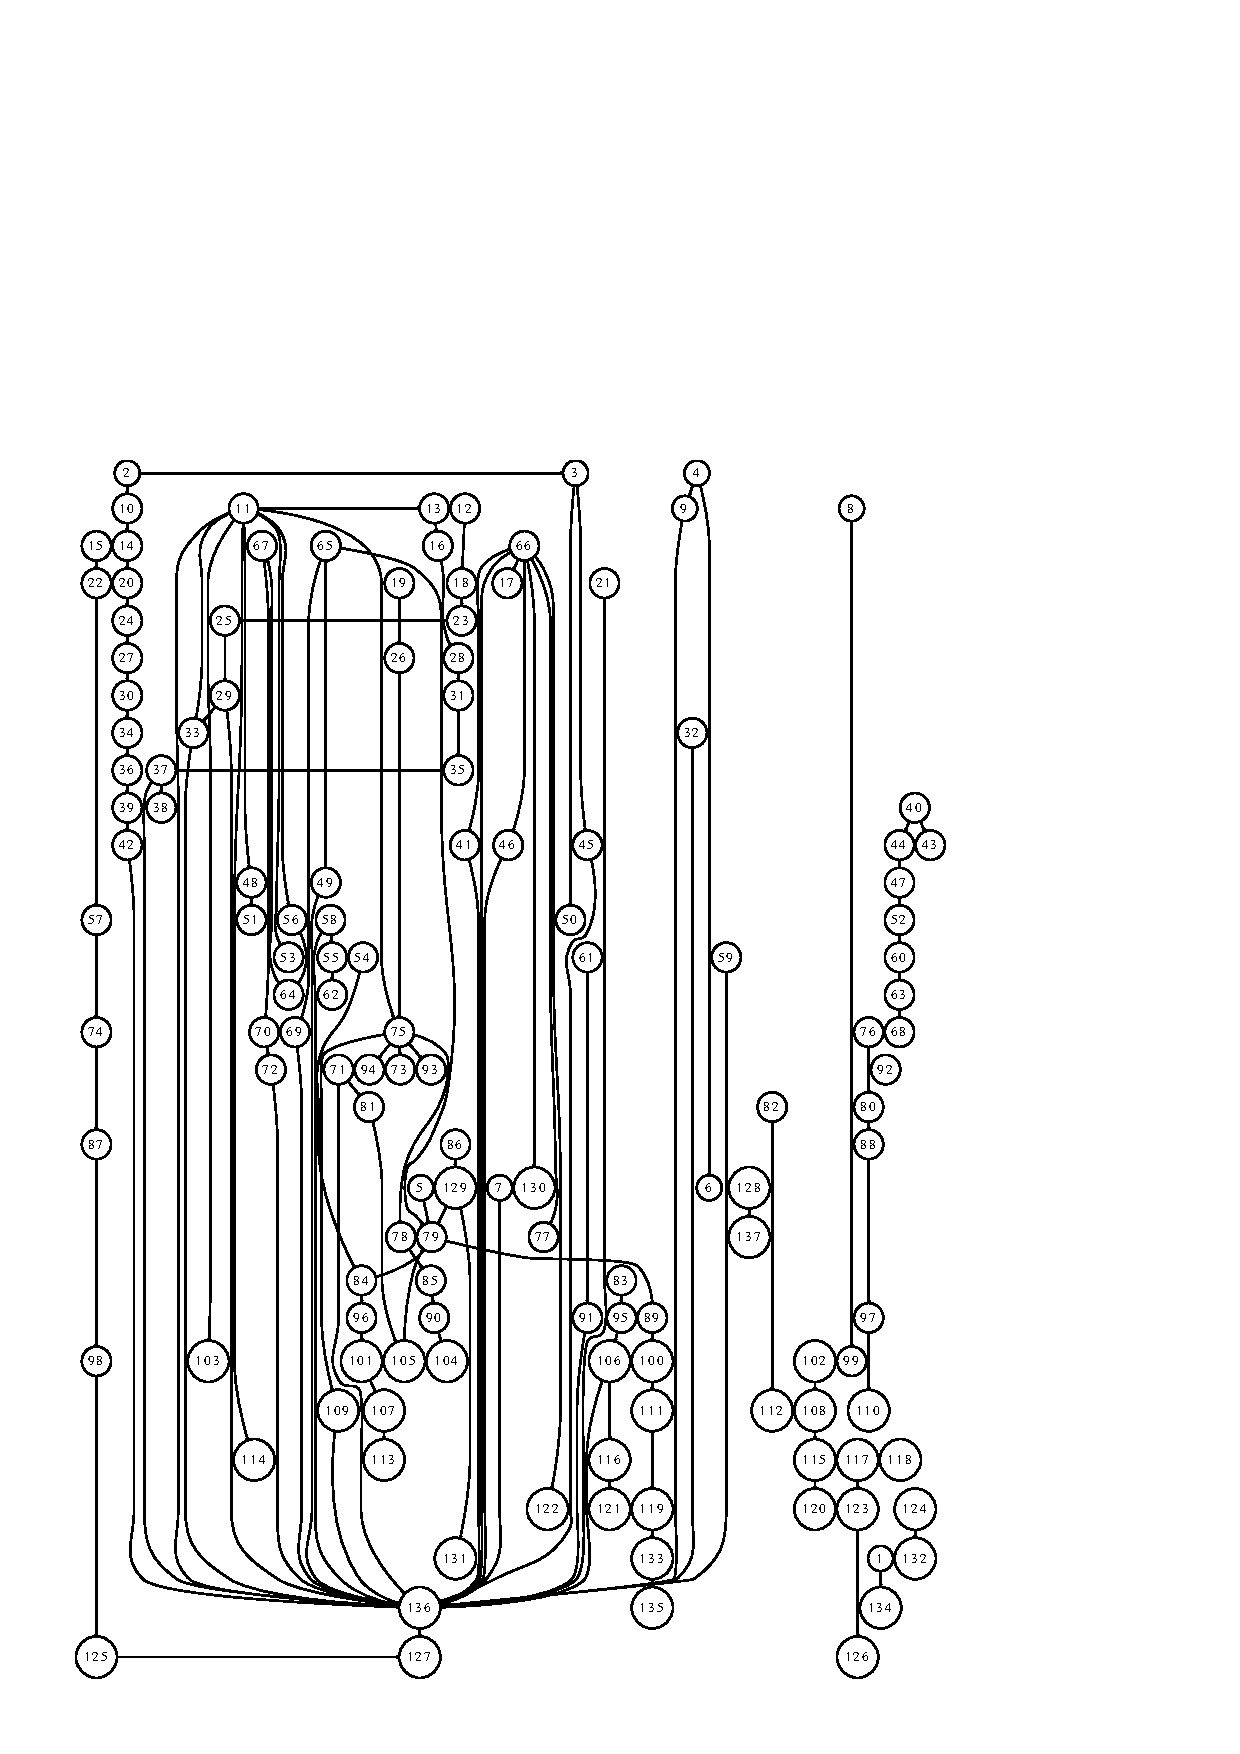
\includepdf{chunks.pdf}

\cleardoublepage

\section*{Notas}

\input{notas.txt}

\cleardoublepage

\section*{Agradecimientos}

\input{agradecimiento.txt}

%%%FOR PRINT
%\cleardoublepage

%\input{pie.txt}

%\includepdf{empty.pdf}
%%%%%%%%%%%%
\end{document}
